%%%%%%%%%%%%%%%%%%%%%%%%%%%%%%%%%%%%%%%%%
% Masters/Doctoral Thesis 
% LaTeX Template
% Version 2.4 (22/11/16)
%
% This template has been downloaded from:
% http://www.LaTeXTemplates.com
%
% Version 2.x major modifications by:
% Vel (vel@latextemplates.com)
%
% This template is based on a template by:
% Steve Gunn (http://users.ecs.soton.ac.uk/srg/softwaretools/document/templates/)
% Sunil Patel (http://www.sunilpatel.co.uk/thesis-template/)
%
% Template license:
% CC BY-NC-SA 3.0 (http://creativecommons.org/licenses/by-nc-sa/3.0/)
%
%%%%%%%%%%%%%%%%%%%%%%%%%%%%%%%%%%%%%%%%%

%----------------------------------------------------------------------------------------
%	PACKAGES AND OTHER DOCUMENT CONFIGURATIONS
%----------------------------------------------------------------------------------------

\documentclass[
11pt, % The default document font size, options: 10pt, 11pt, 12pt
%oneside, % Two side (alternating margins) for binding by default, uncomment to switch to one side
english, % ngerman for German
singlespacing, % Single line spacing, alternatives: onehalfspacing or doublespacing
%draft, % Uncomment to enable draft mode (no pictures, no links, overfull hboxes indicated)
%nolistspacing, % If the document is onehalfspacing or doublespacing, uncomment this to set spacing in lists to single
%liststotoc, % Uncomment to add the list of figures/tables/etc to the table of contents
%toctotoc, % Uncomment to add the main table of contents to the table of contents
%parskip, % Uncomment to add space between paragraphs
%nohyperref, % Uncomment to not load the hyperref package
headsepline, % Uncomment to get a line under the header
%chapterinoneline, % Uncomment to place the chapter title next to the number on one line
%consistentlayout, % Uncomment to change the layout of the declaration, abstract and acknowledgements pages to match the default layout
]{MastersDoctoralThesis} % The class file specifying the document structure
\usepackage{rotating}
\usepackage[utf8]{inputenc} % Required for inputting international characters
\usepackage[T1]{fontenc} % Output font encoding for international characters
\usepackage{palatino} % Use the Palatino font by default
%\usepackage[backend=biber, style=apacite, citestyle=numeric-comp, maxcitenames=5, natbib=true, doi=false, eprint=false, url=false, isbn=false]{biblatex} % Use the bibtex backend with the authoryear citation style (which resembles APA)
\usepackage[backend=biber, style=ieee, citestyle=numeric-comp, natbib=true, maxcitenames=5, doi=false, eprint=false, url=false, isbn=false]{biblatex}

\addbibresource{example.bib} % The filename of the bibliography
\usepackage[autostyle=true]{csquotes} % Required to generate language-dependent quotes in the bibliography
\usepackage[final]{pdfpages}
\usepackage{tabu}
\usepackage{tabularx}
\usepackage{amssymb}
\usepackage{mathtools}
\usepackage{dsfont}
\usepackage{multicol}
\usepackage{relsize}
\usepackage{amsmath}
\usepackage{algorithm}
\usepackage[noend]{algpseudocode}
\usepackage{framed}
\usepackage{array}
\usepackage{caption}
%\captionsetup[table]{skip=10pt}
\usepackage{subcaption}
\usepackage{graphicx}
\usepackage{multirow}
\usepackage{siunitx}
\usepackage{color}
\usepackage{listings}
\usepackage{longtable}
\usepackage{setspace}
\newcolumntype{L}{>{\arraybackslash}p{0.7\textwidth}}
\newcolumntype{G}{>{\arraybackslash}p{0.3\textwidth}}
\usepackage{tikz}
\usetikzlibrary{shapes,arrows}
\usepackage{verbatim}
\usepackage{tensor}
\definecolor{Code}{rgb}{0,0,0}
\definecolor{Decorators}{rgb}{0.5,0.5,0.5}
\definecolor{Numbers}{rgb}{0.5,0,0}
\definecolor{MatchingBrackets}{rgb}{0.25,0.5,0.5}
\definecolor{Keywords}{rgb}{0,0,1}
\definecolor{self}{rgb}{0,0,0}
\definecolor{Strings}{rgb}{0,0.63,0}
\definecolor{Comments}{rgb}{0,0.63,1}
\definecolor{Backquotes}{rgb}{0,0,0}
\definecolor{Classname}{rgb}{0,0,0}
\definecolor{FunctionName}{rgb}{0,0,0}
\definecolor{Operators}{rgb}{0,0,0}
\definecolor{Background}{rgb}{0.98,0.98,0.98}
\lstdefinelanguage{Python}{
numbers=left,
numberstyle=\footnotesize,
numbersep=1em,
xleftmargin=1em,
framextopmargin=2em,
framexbottommargin=2em,
showspaces=false,
showtabs=false,
showstringspaces=false,
frame=l,
tabsize=4,
% Basic
basicstyle=\ttfamily\small\setstretch{1},
backgroundcolor=\color{Background},
% Comments
commentstyle=\color{Comments}\slshape,
% Strings
stringstyle=\color{Strings},
morecomment=[s][\color{Strings}]{"}{"},
morecomment=[s][\color{Strings}]{'}{'},
% keywords
morekeywords={import,from,class,def,for,while,if,is,in,elif,else,not,and,or,print,break,continue,return,True,False,None,access,as,,del,except,exec,finally,global,import,lambda,pass,print,raise,try,assert},
keywordstyle={\color{Keywords}\bfseries},
% additional keywords
morekeywords={[2]@invariant,pylab,numpy,np,scipy,matplotlib,pyplot,pl,mpl_toolkits,mplot3d,Axes3D,math,random },
keywordstyle={[2]\color{Decorators}\slshape},
emph={self},
emphstyle={\color{self}\slshape},
%
}
\tikzstyle{block} = [draw, fill=blue!20, rectangle, 
    minimum height=3em, minimum width=6em]
\tikzstyle{sum} = [draw, fill=blue!20, circle, node distance=1cm]
\tikzstyle{input} = [coordinate]
\tikzstyle{output} = [coordinate]
\tikzstyle{pinstyle} = [pin edge={to-,thin,black}]


%----------------------------------------------------------------------------------------
%	MARGIN SETTINGS
%----------------------------------------------------------------------------------------

\geometry{
	paper=a4paper, % Change to letterpaper for US letter
	inner=2.5cm, % Inner margin
	outer=3.8cm, % Outer margin
	bindingoffset=.5cm, % Binding offset
	top=1.5cm, % Top margin
	bottom=1.5cm, % Bottom margin
	%showframe, % Uncomment to show how the type block is set on the page
}

%----------------------------------------------------------------------------------------
%	THESIS INFORMATION
%----------------------------------------------------------------------------------------

%\thesistitle{Distance Based Formation Control of Three Robotic Arms} % Your thesis title, this is used in the title and abstract, print it elsewhere with \ttitle
%\supervisorone{prof. dr. Bayu Jayawardhana} % Your first supervisor's name, this is used in the title page, print it elsewhere with \supnameone
%\supervisortwo{prof. dr. ir. Ming Cao} % Your first supervisor's name, this is used in the title page, print it elsewhere with \supnametwo
\examiner{} % Your examiner's name, this is not currently used anywhere in the template, print it elsewhere with \examname
\degree{Industrial Engineering and Management} % Your degree name, this is used in the title page and abstract, print it elsewhere with \degreename
\author{Wiljan Vos} % Your name, this is used in the title page and abstract, print it elsewhere with \authorname
\addresses{Koolstraat 17, Groningen} % Your address, this is not currently used anywhere in the template, print it elsewhere with \addressname
\keywords{} % Keywords for your thesis, this is not currently used anywhere in the template, print it elsewhere with \keywordnames
\university{University of Groningen} % Your university's name and URL, this is used in the title page and abstract, print it elsewhere with \univname
\faculty{Faculty of Science and Engineering} % Your faculty's name and URL, this is used in the title page and abstract, print it elsewhere with \facname

%\AtBeginDocument{
%\hypersetup{pdftitle=\ttitle} % Set the PDF's title to your title
%\hypersetup{pdfauthor=\authorname} % Set the PDF's author to your name
%\hypersetup{pdfkeywords=\keywordnames} % Set the PDF's keywords to your keywords
%}

\begin{document}


\frontmatter % Use roman page numbering style (i, ii, iii, iv...) for the pre-content pages

\pagestyle{plain} % Default to the plain heading style until the thesis style is called for the body content

%----------------------------------------------------------------------------------------
%	TITLE PAGE
%----------------------------------------------------------------------------------------

\begin{titlepage}
\begin{center}

\vspace*{.06\textheight}
{\scshape\LARGE University of Groningen\par}\vspace{1.5cm} % University name
\textsc{\Large Master Design Project}\\[0.5cm] % Thesis type
\textsc{\large Industrial Engineering and Management}\\[0.5cm]

\HRule \\[0.4cm] % Horizontal line
{\huge \bfseries Design of a Condition-Based Maintenance Tool for Beenen B.V. - concept\par}\vspace{0.4cm} % Thesis title
\HRule \\[1.5cm] % Horizontal line
 
\begin{minipage}[t]{0.4\textwidth}
\begin{flushleft} \large
\emph{Author:}\\
{Wiljan F. Vos} % Author name - remove the \href bracket to remove the link
\end{flushleft}
\end{minipage}
\begin{minipage}[t]{0.4\textwidth}
\begin{flushright} \large
\emph{University supervisors:} \\
{dr. Gunn K. H. Larsen} \\% Supervisor name - remove the \href bracket to remove the link
{prof. dr. Bayu Jayawardhana} \\ [0.5cm]
\emph{Company supervisor:} \\
{Thom Verwater} \\
\end{flushright}
\end{minipage}\\[1cm]


\includegraphics[width=0.45\textwidth]{Figures/rugr_logoen_rood_rgb}\\[0.25cm]

\includegraphics[width=0.45\textwidth]{Figures/Beenen-logo}\\[0.3cm]% University/department logo - uncomment to place it

\vfill
\textsc{\large Faculty of Science and Engineering}\\ % Research group name and department name

\vfill
{\large \today} % Date
 
\vfill
\end{center}
\end{titlepage}

%----------------------------------------------------------------------------------------
%	ABSTRACT PAGE
%----------------------------------------------------------------------------------------

\begin{abstract}

TBD\\
\textbf{Purpose:} Why do we care about the problem? What practical, scientific, theoretical or artistic gap is your research filling? Start with: 'The purpose of this paper...' or 'This paper aims to...'. \\
\textbf{Method:} What did you actually do to get your results? For example: Analyzed 3 novels, completed a series of 5 oil paintings, interviewed 17 students.\\
\textbf{Findings:} As a result of completing the above procedure, what did you learn/invent/create? This will refer to analysis, discussion, or results.\\
\textbf{Implications:} What are the larger implications of your findings, especially for the problem/gab identified in step 1?\\
\textbf{Value:} What is new in the paper? State the value of the paper and to whom.
\end{abstract}

%----------------------------------------------------------------------------------------
%	ACKNOWLEDGEMENTS
%----------------------------------------------------------------------------------------

\begin{acknowledgements}
Acknowledgements
\end{acknowledgements}
%----------------------------------------------------------------------------------------
%	LIST OF CONTENTS/FIGURES/TABLES PAGES
%----------------------------------------------------------------------------------------
\setcounter{tocdepth}{2}
\newcommand{\newcontentsname}{Contents}
\renewcommand{\cfttoctitlefont}{%
    \begin{flushleft}
    \checktoopen
		\LineRule \\[0.1cm] % Horizontal line
		{\huge \newcontentsname\par} % Thesis title
		\LineRule \\[0.1cm] % Horizontal line
	\end{flushleft}}
\renewcommand{\contentsname}{}
\tableofcontents % Prints the main table of contents

\newcommand{\newlistfigurename}{List of Figures}
\addchaptertocentry{\newlistfigurename}
\renewcommand{\cftloftitlefont}{%
	\newpage
    \begin{flushleft}
		\LineRule \\[0.1cm] % Horizontal line
		{\huge \newlistfigurename\par} % Thesis title
		\LineRule \\[0.1cm] % Horizontal line
	\end{flushleft}}
\renewcommand{\listfigurename}{}
\listoffigures

\newcommand{\newlisttablename}{List of Tables}
\addchaptertocentry{\newlisttablename}
\renewcommand{\cftlottitlefont}{%
    \begin{flushleft}
    \newpage
		\LineRule \\[0.1cm] % Horizontal line
		{\huge \newlisttablename\par} % Thesis title
		\LineRule \\[0.1cm] % Horizontal line
	\end{flushleft}}
\renewcommand{\listtablename}{}
\listoftables % Prints the list of tables

%----------------------------------------------------------------------------------------
%	ABBREVIATIONS
%----------------------------------------------------------------------------------------

\begin{abbreviations}{ll} % Include a list of abbreviations (a table of two columns)
\newcommand{\newabbreviationname}{List of Abbreviations}
\addchaptertocentry{\newabbreviationname} \\
\textbf{AL} & \textbf{A}ssembly \textbf{L}ine \\
\textbf{APV} & \textbf{A}utomatische \textbf{P}rintplaat \textbf{V}erwerking \\
\textbf{BBA} & \textbf{B}asic \textbf{B}ody \textbf{A}ssembly \\
\textbf{BSD} & \textbf{B}usiness \textbf{S}ystem \textbf{D}esign \\
\textbf{CBM} & \textbf{C}ondition \textbf{B}ased \textbf{M}aintenance \\
\textbf{CM} & \textbf{C}orrective \textbf{M}aintenance\\
\textbf{CMMS} & \textbf{C}omputerized \textbf{M}aintenance \textbf{M}anagement \textbf{S}ystem \\
\textbf{CUSTO} & \textbf{Custo}mization \\
\textbf{DI} & \textbf{D}egradation \textbf{I}ndicator \\
\textbf{DUM} & \textbf{D}riving \textbf{U}nit \textbf{A}ssembly \\
\textbf{HCA} & \textbf{H}air \textbf{C}hamber \textbf{A}ssembly \\
\textbf{HMI} & \textbf{H}uman \textbf{M}achine \textbf{I}nterface\\
\textbf{JIT} & \textbf{J}ust \textbf{I}n \textbf{T}ime\\
\textbf{KOR} & \textbf{K}nowledge \textbf{O}riented \textbf{R}esearch \\
\textbf{MCSA} & \textbf{M}otor \textbf{C}urrent \textbf{S}ignature \textbf{A}nalysis \\
\textbf{OG} & \textbf{O}ndersteundende \textbf{G}roep\\
\textbf{OTD} & \textbf{O}nderhoud \textbf{T}echnische \textbf{D}ienst \\
\textbf{PCA} & \textbf{P}rincipal \textbf{C}omponent \textbf{A}nalysis \\
\textbf{PDF} & \textbf{P}robability \textbf{D}ensity \textbf{F}unction \\
\textbf{POR} & \textbf{P}ractice \textbf{O}riented \textbf{R}esearch \\
\textbf{RAC} & \textbf{R}obot \textbf{A}ssembly \textbf{C}ell\\
\textbf{R\&D} & \textbf{R}esearch \textbf{}and \textbf{D}evelopment\\
\textbf{RUL} & \textbf{R}emaining \textbf{U}seful \textbf{L}ife\\
\textbf{SCARA} & \textbf{S}elective \textbf{C}ompliance \textbf{A}ssembly \textbf{R}obot \textbf{A}rm\\
\textbf{SUA} & \textbf{S}have \textbf{U}nit \textbf{A}ssembly \\
\textbf{TBM} & \textbf{T}ime \textbf{B}ased \textbf{M}aintenance\\
\textbf{WT} & \textbf{W}erk \textbf{T}räger \\
\end{abbreviations}

%----------------------------------------------------------------------------------------
%	PHYSICAL CONSTANTS/OTHER DEFINITIONS
%----------------------------------------------------------------------------------------

%\begin{constants}{lr@{${}={}$}l} % The list of physical constants is a three column table

% The \SI{}{} command is provided by the siunitx package, see its documentation for instructions on how to use it
%Example:\\
%Speed of Light & $c_{0}$ & \SI{2.99792458e8}%{\meter\per\second} (exact)\\
%Constant Name & $Symbol$ & $Constant Value$ with units\\

%\end{constants}

%----------------------------------------------------------------------------------------
%	SYMBOLS
%----------------------------------------------------------------------------------------

%\begin{symbols}{lll} % Include a list of Symbols (a three column table)
%Example:\\
%$a$ & distance & \si{\meter} \\
%$P$ & power & \si{\watt} %(\si{\joule\per\second}) \\
%Symbol & Name & Unit \\

%\addlinespace % Gap to separate the Roman symbols from the Greek

%$\omega$ & angular frequency & \si{\radian} \\

%\end{symbols}

%----------------------------------------------------------------------------------------
%	THESIS CONTENT - CHAPTERS
%----------------------------------------------------------------------------------------

\mainmatter % Begin numeric (1,2,3...) page numbering

\pagestyle{scrheadings} % Return the page headers back to the "thesis" style

% Include the chapters of the thesis as separate files from the Chapters folder
% Uncomment the lines as you write the chapters

% Chapter 1

\chapter{Introduction} % Main chapter title

\label{Chapter1} % For referencing the chapter elsewhere, use \ref{Chapter1} 

%----------------------------------------------------------------------------------------

% Define some commands to keep the formatting separated from the content 
\newcommand{\keyword}[1]{\textbf{#1}}
\newcommand{\tabhead}[1]{\textbf{#1}}
\newcommand{\code}[1]{\texttt{#1}}
\newcommand{\file}[1]{\texttt{\bfseries#1}}
\newcommand{\option}[1]{\texttt{\itshape#1}}

%----------------------------------------------------------------------------------------

\section{Business context} \label{Business context}
This design project is originated from Beenen B.V. in Heerenveen, an industrial automation company that designs and constructs entire control systems for industry, infrastructure and water-technology. With more than 200 employees, divided over the locations Heerenveen, Zwolle and Nijkerk, they execute projects national and international. After delivery, Beenen provide maintenance, support, and inspections to their customers. This maintenance support includes the software inspection and repair of equipment and installations but also services to improve the systems. Currently, this support and service is performed on-site by engineers employed at Beenen Heerenveen or Zwolle. Beenen has customers located worldwide that construct and deliver installations with control systems designed by Beenen. Companies in Russia, South-Africa, Brazil and Mexico among others use machines with control systems designed by Beenen. If an installation breaks down and maintenance is required, the needed knowledge to repair is not available on-site in that foreign country. Many installations are able to log and transmit data and therefore it should not be necessary to provide on-site support to maintenance teams. Analyzing data derived from the control systems makes it possible to assist customer maintenance teams worldwide. For this reason, centralizing maintenance at Heerenveen or Zwolle is one of the management goals.

Furthermore, the collected data from customers lend itself for further analysis and processing. For example, an application of predictive maintenance may be possible for customer installations. Predictive maintenance, also called condition-based maintenance (CBM) will be discussed extensively in Section \ref{Literature review}. For now, it can be seen as a tool that can predict upcoming necessary maintenance and therefore reduce unplanned downtime and decreasing total maintenance cost. Beenen tries to decrease the cost of ownership for customers by adding these features to their products. For now, Beenen is not allowed to collect data from customers since the data it is not their property. To be able to provide CBM to their products and services a collaboration with one of their customers, that allows making use of their data, is necessary. The search for a customer that is willing to develop a CBM tool in collaboration with the Research and Development (R\&D) department from Beenen lead to Philips Consumer Lifestyle B.V. in Drachten. Beenen has  established service contracts with Philips Drachten and software engineers are already deployed there. This makes Philips a very useful company to collaborate with in order to obtain production data that can be used by designing a CBM tool. 

Philips Drachten is a developer of numerous innovative products such as shavers, trimmers, vacuum cleaners and coffee machines. The location site at Drachten has 2000 employees, including 600 developers\footnote{https://en.icdrachten.nl/companies/philips}. This project is focused on the maintenance department of the shaver production process. Philips Drachten develops and produces the shaving heads for all Philips shavers, high-end and mid-range shavers. The shaver assembly department consist of multiple assembly lines (AL), where every line is established to assemble one type of shaver. The shaver ALs are divided over 3 mini-companies called Cypress, Thor and Better-Best, producing the 9000 series, 3000 series and 5000 and 7000 series, respectively. Since mini-company Thor features the oldest installations in comparison with the other mini-companies, upcoming maintenance is expected here firstly and this design project will focuses on the ALs at Thor.

To provide context to the rest of this thesis, an overview of how the shavers at Philips are produced is given next. All shaver types, mentioned in the previous section, are assembled by multiple robot assembly cells (RAC)s placed in line in large factory halls. RACs consist of robotic arms, feeders, vision cameras and specific conveyor belts. The maintenance department, consisting of OTD and OG, is responsible for all maintenance that is necessary for those ALs. Every single shaver is assembled by multiple lines that are divided in the following groups: Hair Chamber Assembly (HCA), Shaver Unit Assembly (SUA), Driving Unit Mechanization (DUM), Basic Body Assembly (BBA), Customization (CUSTO) and Automatic Printed circuit board Process, in dutch: Automatische Printplaat Verwerking (APV). In Figure \ref{fig:assemblyline} it is shown how the different lines are ordered within mini-company Thor. After testing the shavers in the CUSTO, shipment takes place from Drachten to Hungary where the shavers will be packaged and distributed over the global market. The aim of this research is to explore CBM for the robot arms in Thor and therefore not all various types of ALs and RACs are discussed in detail. However, all mentioned abbreviations will be used often in this thesis and are therefore of importance.
\begin{figure}[ht]
\centering
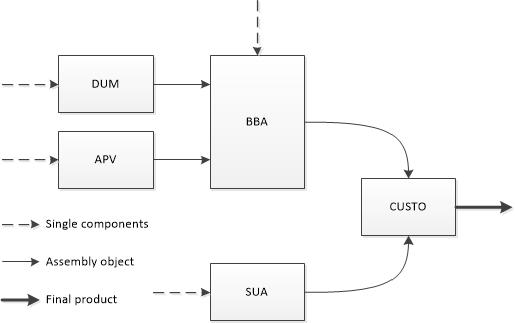
\includegraphics[width=\textwidth]{Figures/assemblyline_Thor}
\caption[Overview of mini-company Thor with corresponding types of ALs]{Overview of mini-company Thor with corresponding types of ALs}
\label{fig:assemblyline}
\end{figure}

\section{Problem context} \label{Problem Context}
Thor's desired production rate is already at a maximum production capacity of 120.000 products per week, which is equal to 1000 products per hour. In comparison, Better-Best and Cypress produce at 70\% and 50\% of their production capacity, respectively. To ensure that an AL is not running out of assembly objects, buffers between every AL are established. The buffer is a storage location, indicated with lines on the floor and info cards, where carts are stored with a maximum capacity of 6 carts. The carts have a capacity of 45 trays, each with 16 place holders, and therefore 720 assembly objects per cart and 4320 per buffer location. The operators of an AL are responsible for placing the carts from the last RAC of an AL, the supplier, to the buffer location and from there to the first RAC of the next AL, the customer, on a First In First Out basis. If maintenance is performed at one AL, the other ALs are continuing  production until the maximum buffer capacity is reached or carts are empty and no assembly objects are available. The last case will result in losses since no assembly objects are arriving at the CUSTO and are finalized. To prevent this from happening, the maintenance department of Philips has the primary task to keep the production running with minimal failures and downtime. Failures can be seen not only as breakdown of equipment but also as other events where maintenance is performed at an AL. For example, lubricating the joints of a robot arm. 
%\textbf{(1) Direct Costs:}\\
%Labour
%\begin{itemize}
%\item Normal and overtime labor for
%{\setlength\itemindent{15pt} \item planned repair activities}
%{\setlength\itemindent{15pt} \item unplanned repairs}
%\end{itemize}
%Materials
%\begin{itemize}
%\item Parts replaced
%\item Machinery replaced\\
%\end{itemize}
%\textbf{(2) Indirect Costs:}
%\begin{itemize}
%\item Lost production (€/hour)
%\item Outside services
%\item Insurance costs
%\item Parts inventory
%\end{itemize}
%\textbf{Total Potential Cost Reduction (1+2)}\\
%\\
%\\
%\textbf{(3) PdM Program Costs}
%\begin{itemize}
%\item Site survey
%\item Cost of capital equipment
%\item Cost of any additional labor
%\item Cost of training
%\item Initial setup and baseline
%\item Scheduled data collection 
%\end{itemize}
%\textbf{Total PdM costs for one year (3)}\\

Currently, maintenance on the RACs is performed after a breakdown or failure occurs. This type of maintenance is called corrective maintenance (CM) and will be discussed and compared briefly with other maintenance strategies in Section \ref{Literature review}. The RAC will be disassembled and mechanics from the OTD will investigate what the problem is and how to repair it. Depending on the type of maintenance this can be an extensive and time-consuming task. For example, if a harmonic drive of a robot arm is broken, it takes on average 2-4 hours to replace a robot arm. Since Thor's production rate is already at the maximum, this downtime cannot be overcome and 2000-4000 less products can be produced. This amount of products should be produced in overtime, for example during weekends. As for every company, this overtime is costly and needs to be avoided. Stopping the AL will result in €152,- per hour extra costs.  

Furthermore, an aforementioned harmonic drive has 4 weeks of delivery time and therefore the maintenance department has a few spare parts. This inventory should be kept as low as possible since that the harmonic drives are very costly, €5000,- each. Due to the low amount of spare harmonic drives, a breakdown of multiple harmonic drives around the same time can therefore be catastrophic for the maintenance department of Thor. 

The problem is that there is no efficient maintenance schedule available at Philips and therefore to minimize the inventory and maximize the production rate, one of the maintenance department objectives is to provide an efficient maintenance schedule for their installations. They strive to predict maintenance before failure and adjust the maintenance planning based on that prediction. Similar to the management of Beenen, the maintenance department of Philips has the objective to add CBM to their installations and control systems. 

\section{Research approach} \label{Research approach}
\subsection{Practice oriented research}
Every research or design project aims to provide knowledge, insight and information that can contribute towards solving a problem that can be distinguished into knowledge problems and practical problems \parencite{Verschuren2010}. Where knowledge oriented research (KOR) focuses on knowledge problems by adding knowledge to the knowledge base and practice oriented research (POR) focuses on designing an artifact to solve a practical problem. For this project the problem as described before about the maintenance schedule is of practical nature. To design an artifact, literature have to be reviewed, elaborated and will be used during the design. For this project, no new scientific knowledge will be added to the knowledge base if the maintenance schedule is improved. However, by adding CBM to the RACs and performing experiments new knowledge can be obtained that contributes to the knowledge base. Nevertheless, this project will be considered as POR since obtaining new knowledge is not relevant to the maintenance department of Philips nor the R\&D department of Beenen.

\subsection{The Regulative cycle} \label{The Regulative Cycle}
The regulative cycle is a practice oriented research method that is most useful by design projects. In contradiction, the empirical cycle focuses on knowledge oriented research. The regulative cycle has been applied extensively as a methodology and is formulated by van \citet{vanStrien1986}. It contains the five phases depicted in Figure \ref{fig:Regulative cycle} and described below:
\begin{figure}[ht]
\centering
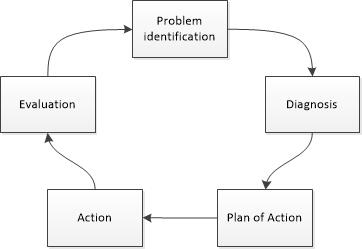
\includegraphics[]{Figures/Regulative_Cycle}
\caption[Regulative cycle]{Regulative cycle based on van Strien \parencite{vanStrien1986,vanStrien1997}}
\label{fig:Regulative cycle}
\end{figure}
\begin{itemize}
\item \textit{Problem identification}; Determines what the exact problem is, why it is a problem and whose problem it is. A specific problem could be defined in order to help with the accurate execution of the research.
\item \textit{Diagnosis}; Examines background and causes of the identified problem. A plan of action can only be formulated if the reason for the problem is understood.
\item \textit{Plan of Action}; Formulates how the problem should be solved by setting up a artifact design.
\item \textit{Action}; Interference of the plan of action formulated in the previous phase. The artifact is applied to the system in order to solve the problem.
\item \textit{Evaluation}; Verifies whether the implemented changes have actually solved the problem. Mostly, the problem is only solved partially and new problems will emerge. The phases described above will then be repeated with the new problems.
\end{itemize}

\subsection{Business System Design} \label{BSD}
The Business System Design (BSD) method, in dutch: OBS method, is a framework formulated by \citet{Prins2008} that describes how to perform the problem identification and diagnosis phases correctly. The diagnosis in BSD is a worked-out approach of the problem identification and diagnosis phase of the regulative cycle. It provides the researcher with a clear guideline throughout these steps of the research. 

The first phase is to address the 'right' problem with corresponding problem owner. This phase is called the problem determining phase and consist of problem owner analysis, system description, stakeholder analysis, problem definition and research goal. After the problem determining phase, the first part of the conceptual research design phase will be addressed where research questions are formulated, literature is reviewed and a conceptual causal model is build. In the second part of the conceptual research design phase, concepts of operationalization, choice of tools and techniques and a data gathering plan are discussed. The problem identification and diagnosis is described in Chapter \ref{Chapter2}. The other phases in the regulative cycle are addressed afterwards. The plan of action that will be executed is constructed in Chapters \ref{Chapter3} and \ref{Chapter4}. The execution will be described in Chapter \ref{Chapter5} and evaluated in Chapter \ref{Chapter6}. A more detailed outline of this thesis will be provide in the next section.

\section{Thesis outline} \label{Thesis outline}
TBD
% Chapter 1

\chapter{Problem Analysis} % Main chapter title

\label{Chapter2} % For referencing the chapter elsewhere, use \ref{Chapter1} 
In this chapter, the problem analysis as described by \citet{Prins2008} in Section \ref{BSD} will be applied. The problem owner will be described, a system description is given, stakeholder analysis is performed and a clear and concise problem definition is formulated. In the end, a research goal that fulfills the stakeholder and problem owner requirements is formulated.

\section{Problem owner analysis} \label{Problem owner analysis}
As mentioned in the previous section, this project is originated from Beenen. The higher management goal is to centralize maintenance support at a Beenen facility in Heerenveen or Zwolle. To accomplishing this goal, an implementation of CBM is desired and therefore have to be designed. Designing this tool requires analyzable data available from control systems and will be obtained in collaboration with Philips. Within Beenen, several employees are connected to the installations at Philips Drachten by providing maintenance support and services. Thom Verwater and Kevin Schipper are the leading R\&D employees aiming for an implementation of CBM to their designed installations and can therefore be seen as the problem owners. 

The maintenance department of Philips will play a big role during this design project. The aimed application of CBM to their RACs will contribute to their objectives, stated in Section \ref{Problem Context}, as well. However, Philips will not be seen as problem owner since the intended output of this design project will be property of Beenen. 

\section{System description} \label{System description}
The initial goal of the problem owners is to design a system that is able to predict upcoming maintenance by analyzing data that is available from their designed control systems. This tool should then be added to the products and services Beenen offers. It indicates that the investigated system is a maintenance decision making system that consist of input, output, external factors and subsystems. Focusing on the Philips case, data, such as currents, torques, temperatures and positions errors, available from the RACs can then be seen as the input for the maintenance system and a maintenance schedule as the output. Subsystems within the boundaries of the system are the functions: data logging, comparing limit values and schedule compiling. Activities as performing maintenance and ordering inventory are outside the scope of this project and are therefore not within the boundaries of the described system. A diagram of the system description with corresponding input, output and subsystems can be seen in Figure \ref{fig:System_Description}. 
\begin{figure}[ht]
\centering
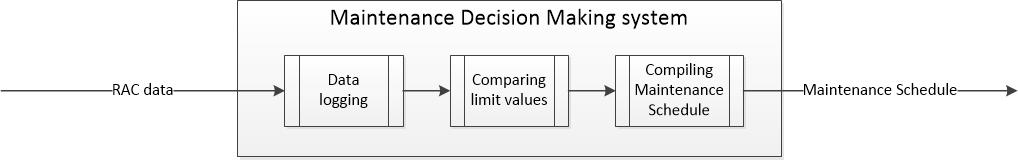
\includegraphics[width=\textwidth]{Figures/Intended_System_Description}
\caption[General system description]{A general system description with corresponding input, output and subsystems.}
\label{fig:System_Description}
\end{figure} 

Applying CBM to all installations at Philips Drachten will be an extensive and complex task. Executing such a project is therefore not realistic in the available time for this project. Therefore, this project focuses on one specific RAC only. Implementing the design on the control system of the RAC is done by software engineers at Beenen and therefore outside the system-boundaries of this project. 

However, it would be possible to shift the boundaries and expand the number of RACs. The number of maintenance actions, feasibility, and related maintenance costs are examples of performance indicators that determine the appropriateness of applying CBM to a specific cell. This indicators are judged by Philips employees that have experience with the installations.

This system description is generic written because the aimed CBM tool as described in Section \ref{Business context} should be applied to all control systems Beenen designs or maintains, in the end. Nevertheless, from interviews with members of the OG and OTD it is discussed to focus this design project on RAC RB34. One of the Robot Arms within this cell leaks some oil and upcoming maintenance is expected, therefore it is suitable to investigate the data regarding this cell. A description of this cell is given in Section \ref{RB34 description} and the entire process description (dutch) can be found in Appendix \ref{AppendixA}. 

\subsection{Description of RAC RB34} \label{RB34 description}
RB34 is part of AL SUA3 that assembles the shaver unit of mini-company Thor, the 3000 series shaver. Other RACs that are part of SUA3 are RB31, RB32, RB33, RB35 and TF135. Where the RB cells are all responsible for assembling a different part of the shaver unit from the 3000 series and the TF cell is responsible for feeding trays to RB35 carrying parts that are assembled to the shaver unit. A double conveyor belt ensures a continuous flow of product carriers, in deutsch: Werk Trägers (WT)s and in dutch: productdragers, that support the assembly objects. 

Firstly, the assembly objects arrive in RB34 on WTs from RB33 at the first position and Robot Arm 1, a Adept Cobra\textsuperscript{\tiny{TM}} s600, assembles the holder springs, see Figure \ref{fig:Holder springs}, to the assembly object. Thereafter, the WT moves to the second position in RB34 and Robot Arm 2, also a Cobra s600, assembles the Holders, see Figure \ref{fig:Holders}. The holder springs and Holders are equal for every shaver unit of Thor. Via a sensor, the presence of a holder spring and a WT at position 1 or 2 is detected. Additional, a scrap cutter, in dutch: schrot snijder, with conveyor belt provides the Holder Springs to Robot Arm 1.

\begin{figure}[ht]
\centering
\begin{subfigure}[b]{0.49\textwidth}
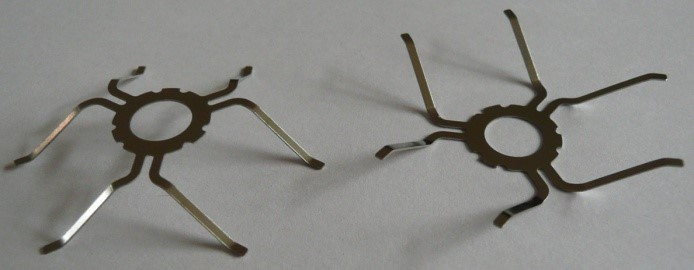
\includegraphics[width=\textwidth, height=3cm]{Figures/Afbeeldin1_Holder_springs}
\caption{Holder springs}
\label{fig:Holder springs}
\end{subfigure}
\begin{subfigure}[b]{0.49\textwidth}
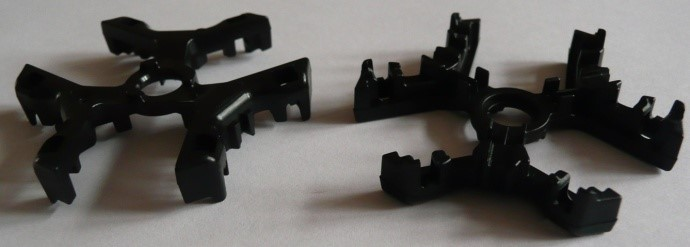
\includegraphics[width=\textwidth, height=3cm]{Figures/Afbeelding2_Holders}
\caption{Holders}
\label{fig:Holders}
\end{subfigure}
\caption[Holder Springs and Holders that are assembled by RB34]{Holder Springs and Holders that are assembled by RB34}
\label{fig:Holders_Holder springs}
\end{figure}

RACs are highly automated and require minimal human supervision during normal operation. In Figure \ref{fig:RACmodel}, it can be seen what inputs and outputs are of a RAC \parencite{Mohamed2001} in the current situation. Inputs are the above described WTs carrying the assembly objects with additional production orders, other inputs are sensors that can detect the holders and springs, spare parts that are necessary during maintenance, programs that control the RAC and tools and fixtures such as the robot arms and feeders. Output of the RAC are the finished products that are transported by conveyor belts to the next RAC where another part of the shaver unit is assembled. Furthermore, feedback on the activities is given by the control system that is integrated to the computer of the RAC in the form of data files. The types of data that are available will be described in Section \ref{Data Gathering}. In the current situation, limit values are not known and therefore it is impossible to determine on forehand which RACs require maintenance according to the data files.
\begin{figure}[ht]
\centering
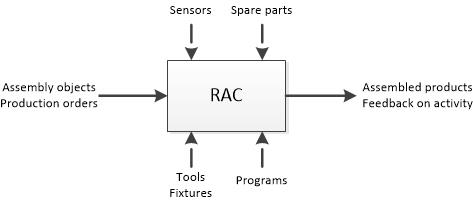
\includegraphics[width=0.7\textwidth]{Figures/RACmodel}
\caption[Model of an RAC]{Model of an RAC}
\label{fig:RACmodel}
\end{figure}

\section{Stakeholder analysis} \label{Stakeholder analysis}
For this design project several stakeholders can be reviewed. The problem owners, Thom Verwater and Kevin Schipper, are the main stakeholders since they want to implement the intended design of this project for their products and services. Those two engineers from Beenen are representing the company and therefore Beenen itself or the director is not be reviewed as stakeholder. Furthermore, the higher management goal of the problem owners is to centralize the maintenance for their customers. In other words, the goal is to generate maintenance schedules at Beenen Heerenveen instead of on-site with live data from the control systems at customers. By scheduling all predictable maintenance for customers a more efficient maintenance system can be obtained. Centralizing all maintenance activities for multiple customers is an extensive task and is not realistic for the time of this project. Therefore, this project focuses on ALs and RACs within mini-company Thor of Phililps Drachten, as mentioned in Section \ref{Business context}.

The maintenance department of Philips Drachten, in particular Maintenance Engineer Dirk Jan Dunsbergen, can also be seen as stakeholder. The project focuses on shaver RACs at Philips and a CBM tool will be designed for these installations. An effective result of this project that can be implemented to these systems will most likely result in a decreasing downtime of the RACs, increasing the throughput-rate of the entire mini-company. Philips Drachten as a company is not reviewed as stakeholder, the same reasoning as applied to Beenen as stakeholder can be applied here. 

A Support Group, in dutch: Ondersteunende Groep (OG), is assigned to one or more mini-companies and consist of the following managers and engineers: Maintenance Engineer, Production Manager, Assistant Production Manager, Quality Manager and Technical Support Mechanic. All of the managers and engineers within this OG are open for questions regarding quality and production of products. However, for this design project, most of them are not of importance since they are not related directly to the maintenance decision making process. Members of the Maintenance Technical Support, in dutch: Onderhoud Technische Dienst (OTD), are responsible for the physical maintenance and repair of RACs and other installations at the AL. Communication with the OTD goes via the Line Mechanic who has a leading function within the OTD and therefore the regular mechanics are not considered as stakeholders. A description of all employees, that are of importance to this project, with corresponding activities and stakes in this project are listed in Table \ref{tab:philips employees}. 

\begin{center}
\begin{longtable}[width=\textwidth]{ p{0.18\textwidth} | p{0.76\textwidth}}
\caption[Stakeholders]{Stakeholders} \vspace{0.3cm} \label{tab:philips employees} \\
Function & Activity/Stake \\ [1ex]
\hline \\
\parbox[t]{0.15\textwidth}{R\&D\\Engineer\\(Beenen)} & Responsible for the R\&D department at Beenen Heerenveen and also the problem owner for this project, see Section \ref{Problem owner analysis} . Strive to improve and develop existing and new products, machines and systems. Furthermore, ensuring smooth transfer of new technologies to other groups within Beenen. By supervising this design project and building further on the aimed CBM tool, the R\&D engineer benefits from this project. \\ [2ex]
\parbox[t]{0.15\textwidth}{Software\\Engineer\\(Beenen)} & Software engineers at Beenen are responsible for development of networks, operating systems, databases and applications. Control systems designed and installed by Beenen need integration of these components. Frank Velthuis is a software engineer working for Beenen at Philips. He is responsible for maintaining and updating the software installed on the RACs. His knowledge can be useful to provide communicating networks between RACs and a higher level system where all available information and data can be combined and processed. Furthermore, the desired CBM tool should be designed partially and integrated in the higher level system by a software engineer. \\ [2ex]
\parbox[t]{0.15\textwidth}{Maintenance\\Engineer\\(Philips)} & Responsible for continuous running of equipment and machinery. Focuses on minimizing downtime by preventing breakdowns and failures. By applying CBM, he aims to reduce the unplanned downtime of all RACs. Conclusions resulting from this project are reviewed and eventually implemented by him. The Maintenance Engineer works closely together with the researcher in order to provide all information regarding maintenance that is necessary to execute the project.  \\ [2ex]
\parbox[t]{0.15\textwidth}{Technical\\Support\\Group\\(Philips)} & Responsible for technical support and problem-shooting for ALs. Focuses on adequate and solid repair of equipment and installations. Works together with software engineers to maintain the systems and keep production running. His knowledge about operating systems can be helpful for the researcher to understand how data available from the RAC can be obtained.\\ [2ex]
\parbox[t]{0.15\textwidth}{Line\\Mechanic\\(Philips)} & Responsible for physical maintaining the production process by ensuring operation of machinery and mechanical equipment. His knowledge about robot arms and other equipment is necessary to determine what maintenance can be predictable. Furthermore, the tasks of the line mechanic can be influenced by implementation of a CBM tool.   \\
\end{longtable}
\end{center}

Stakeholders such as customers of Beenen that are offered installation systems where this design is implemented will not be seen as stakeholders for this project. This is because the stake of those customers correspond to the same objective Beenen has and is not adding extra requirements to the design.

Employees of Beenen that work with the maintenance system can also be considered as stakeholders. Firstly, software engineers need the skills to be able to apply the intended result of this project to their existing products and services. Secondly, other maintenance employees, mechanics and technicians, have to interpret results from the newly designed maintenance system tool in order to perform maintenance. 

\section{Problem definition} \label{Problem definition}
Maintenance performed by Beenen on equipment of customers is handled differently per customer. As mentioned before, this project is a collaboration with Philips and therefore, this project only focuses on the maintenance there. Beenen has a service contract with Philips regarding the software installed on the RACs and ALs. In contrast to other companies, the service contract with respect to Philips state that Beenen is responsible for providing only software support for these ALs. Physical support and maintenance is performed by the OTD of Philips.  

The problem owners, Thom and Kevin from Beenen, want to implement a CBM tool to their products and services to solve the problem of scheduling maintenance for all customers. In the system description this objective is scoped down to the maintenance system at Philips. From this system description it can be concluded that the problem is functional because the problem lays at the output of the system, a lacking maintenance schedule. This schedule is lacking since there is nothing monitored about the condition or average lifetime of the equipment. In this way, it is very hard to predict or prevent upcoming maintenance resulting in unnecessary downtime and high maintenance cost. This makes the problem functional and realistic and therefore the BSD method is applicable to this research project.

The problem statement that can be derived from the information provided by the management and the information stated above and in the previous sections of this chapter is:
\begin{center}
\textit{The use of corrective maintenance to RACs at Philips Drachten causes unplanned downtime, resulting in lower availability of machines than desired.}\\
\end{center}

\section{Design goal} \label{Design goal}
As discussed in Section \ref{Business context} and the previous sections from this chapter, the initial goal of the problem owners is to provide CBM to their designed control systems, helping Beenen to centralize maintenance support. By zooming in to RAC RB34 at Philips a more detailed system description can be provided and a clear and concise goal can be formulated. From this, the design goal of this project can be stated as follows:
\begin{center}
\textit{Improve the maintenance schedule at Philips Drachten for RAC RB34 by designing a CBM tool that satisfies the maintenance requirements and helps Beenen B.V. centralizing maintenance.}\\
\end{center}


%\parencite{Wieringa2014}
%Knowledge questions:\\
%What effects are produced by the interaction between artifact and context?\\
%Do the effects satisfy requirements?

% Chapter Template

\chapter{Research Design} % Main chapter title

\label{Chapter3} % Change X to a consecutive number; for referencing this chapter elsewhere, use \ref{ChapterX}

%----------------------------------------------------------------------------------------
%	SECTION 1
%----------------------------------------------------------------------------------------
\section{Research question}
Design projects iterate over designing and investigating and therefore a research question should be formulated. A research question asks for knowledge about the world, without calling for improvement of the world \parencite{Wieringa2014}. By designing a CBM tool for installations at Philips, it has to be investigated what factors play a role. Therefore, answering the following research question will contribute to the knowledge that is necessary to perform this design project:
\begin{center}
\textit{What factors play a role in applying CBM to the Maintenance Decision Making process of RAC RB34?}\\
\end{center}
In Section \ref{Sub-Questions}, sub-questions are formulated that help to answer the research question and achieve the research goal.

\section{Literature review} \label{Literature review}
Currently, maintenance at the RACs is performed after a machine fails or has broken down. This maintenance strategy is called corrective maintenance (CM) and result in costly repairs since the AL have to be shut down abruptly and the production have to be stopped. The maintenance schedule at Philips contains only little information on the average lifetime of equipment. The goal of this project is to design a CBM tool that replaces the CM and improves the maintenance schedule. However, it is possible that in literature other techniques are more applicable to the installations at Philips Drachten. Therefore, other maintenance techniques are discussed in this literature review as well. First, a description of different maintenance activities is given. Thereafter, the two major maintenance techniques widely discussed in literature are described in more detail: time-based maintenance (TBM) and condition-based maintenance.

%\begin{figure}[ht]
%centering
%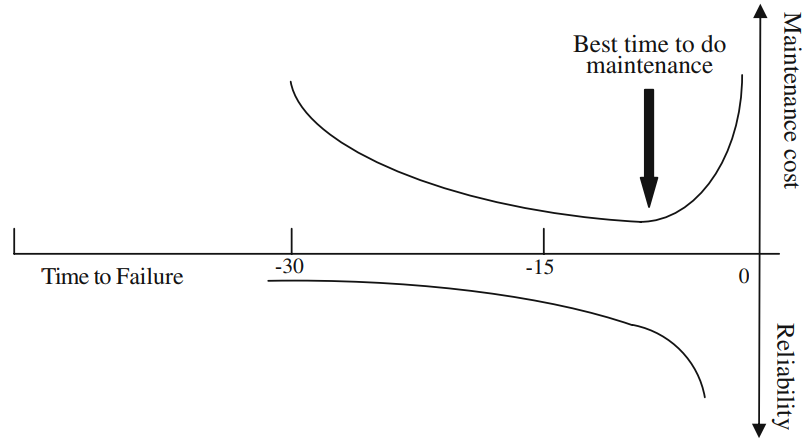
\includegraphics[width=\textwidth, height=7cm]{Figures/bestmaintenance}
%\caption[The relationship between lifetime, reliability, and maintenance cost]{The relationship between lifetime, reliability, and maintenance cost based on \citet{Peng2010}}
%\label{fig:bestmaintenance}
%\end{figure}
\subsection{Introduction to maintenance} \label{Introduction to maintenance}
This introduction to maintenance gives an overview of different possible maintenance activities and is based on lecture nodes for the course Maintenance Planning and Optimization given by Bram de Jonge at the University of Groningen \parencite{DeJonge2017}. 

Organizations are relying more and more on expensive production equipment and therefore the importance of performing maintenance is growing. Nowadays, organizations realize that efficiency and reliability can be improved if maintenance actions are planned more effectively. As a result, the portion of employees working in maintenance is increasing. From a third of the chemical industry employees to a quarter of the process industry employees deal with maintenance operations \parencite{WAEYENBERGH2002}. Therefore, companies in production industries can significantly increase profits by avoiding unplanned stoppages and bad quality production \parencite{ALSYOUF200}. 

Maintenance can be defined as:
\begin{center}
\textit{'All activities necessary to restore equipment to, or keep it in, a state in which it can perform its designated functions'} \parencite{DeJonge2017}.
\end{center}
From this definition it can be deduced that there are two types of maintenance, that is restore equipment or keep it in state. As mentioned before, maintenance performed after a failure or breakdown is called corrective, reactive, or failure-based maintenance. Maintenance performed before a failure or breakdown when the equipment is still functional is called preventive maintenance and aims to prevent or postpone failures. Preventive maintenance is mostly preferred since it can prevent safety issues, machine damage, quality issues, machine unavailability, long repair times and other unplanned maintenance actions. However, performing maintenance too often result in undesirable cost and therefore a balance between preventive maintenance and risk of failure has to be found. In Figure \ref{fig:Maintenance overview} a schematic overview of maintenance strategies is depicted. Preventive maintenance can be divided into TBM, CBM, and Opportunistic maintenance. 

\begin{figure}[ht]
\centering
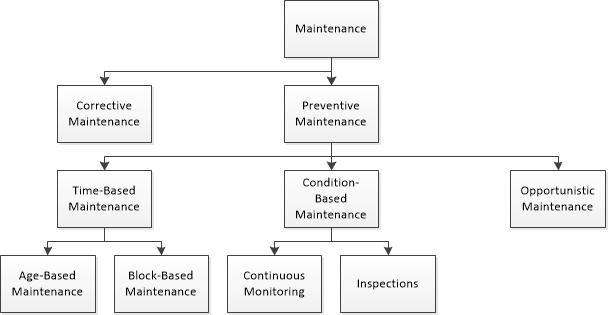
\includegraphics[width=\textwidth]{Figures/Maintenance}
\caption[Schematic overview maintenance strategies]{Schematic overview maintenance strategies based on De Jonge\parencite{DeJonge2017}}
\label{fig:Maintenance overview}
\end{figure}

TBM only depends on the time (age or number of time blocks) that a unit is in service and is therefore relatively easy to implement. However, it is possible that the an item is still in reasonable condition when maintenance is performed or is deteriorating faster than expected and need maintenance earlier. CBM, on the other hand, result in maintenance that is performed just before failure and is generally more effective. However, it can only be applied if condition can be monitored by inspections or continuously and if benefits outweigh the efforts and cost required to apply it. By performing a preventive or corrective maintenance action their might be an opportunity to maintain other units as well. In such cases, the maintenance strategy is called opportunistic. TBM and CBM will be discussed in the next sections, opportunistic maintenance will not be part of this thesis since it can always be combined with another maintenance strategy later. 

\subsection{Time-based maintenance} \label{TBM}
\citet{Yam2001} describe TBM, also known as periodic preventive maintenance, as a traditional maintenance technique. In TBM, maintenance decisions such as preventive repairs are determined based on the estimated expected lifetime of equipment. The expected lifetime is obtained from analyzing the failure behavior of the equipment and, generally, can be displayed as a bathtub curve, Figure \ref{fig:bathtubcurve}. The bathtub curve is divided into three phases: burn-in, useful life, and wear-out. TBM can be introduced to this curve in two steps: The first step is to start with failure data analysis around the left dashed line, the second step is the maintenance decision making at the right dashed line. A complete description of the phases and steps is described by \citet{AHMAD2012}.
\begin{figure}[ht]
\centering
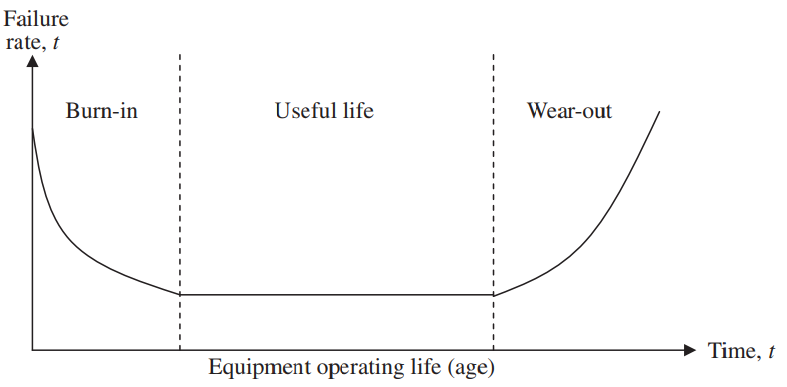
\includegraphics[width=\textwidth]{Figures/bathtubcurve}
\caption[General bathtub curve relation between operating life and failure rate of equipment]{General bathtub curve relation between operating life and failure rate of equipment}
\label{fig:bathtubcurve}
\end{figure}

\citet{GUSTAVSSON2014} consider the scheduling of TBM activities for several components dealing with common set-up costs shared by the components. The gains are combined with the extra costs so that it can be determined if a certain maintenance activity is profitable. TBM contains a number of parameters, such as average lifetime, whose values are optimized numerically or analytically.  However, these parameters are not related to the condition of components but to the estimated lifetime of it. A component far from average can therefore result in performing maintenance too early or too late. A maintenance strategy that is related to the condition of components is discussed below.

\subsection{Condition-based maintenance} \label{CBM}
CBM is thoroughly discussed in literature \parencite{Han2003,AHMAD2012} and is a maintenance program that recommends maintenance decisions based on the condition of equipment and installations. According to \citet{Bloch1983}, 99\% of all machine failures are preceded by certain signs, conditions, or indications that a failure was going to occur. By implementing closed loop maintenance control, sensor feedback information from assembly installations and equipment is utilized in making maintenance-planning decisions. Moreover, continuous collection and interpretation of data regarding the equipment conditions can predict time to failure and an appropriate decision strategy can be applied \parencite{Mann1995}. Firstly, data from various parameters is measured and interpreted continuously, such as vibration, temperature, oil composition, power, and noise levels, which is called the condition monitoring process. This result in maintenance that is performed  just before failure, or just in time (JIT). Secondly, the knowledge of failure causes, effects and deterioration patterns of equipment is increased. Within CBM, diagnostics and prognostics are two important aspects where diagnostics are used for detection, location and identification of faults that occur and prognostics are used to predict the faults before it occurs \parencite{JARDINE2006}. Furthermore, \citet{JARDINE2006} and \citet{Goyal2017} describe that a CBM program consists of three key steps that will be elaborated on briefly: Data acquisition, Data processing, and Maintenance decision making.

\subsubsection{Data acquisition}
Acquiring data is the first step in implementing a CBM program for fault diagnostics and prognostics.  This data can be categorized into event-data and condition monitoring data. Event-data is a description of what happened, for example breakdown, oil pollution or installation and what is done to restore it, for example repair, preventive maintenance or oil replacement. Condition monitoring data are measurements related to the condition health/state of the equipment and installations. As mentioned above there is a wide variety of possible condition monitoring data with as many sensors. The data can be obtained continuously or by inspections. Within seconds, \citet{Golmakani2011} describe an age-based inspection approach where at each step, based on the age of the system, the best time for next inspection is determined. Furthermore, wireless technologies, such as Bluetooth, result in a cost-effective solution to data communication and computerized maintenance management systems (CMMS) are developed for data storage and handling. 

\subsubsection{Data processing}
After the acquisition of data it have to be processed. First, the data is cleaned from any noise preventing it from containing errors, see Section \ref{Data cleaning}. Nevertheless, data cleaning is more applicable to event-data than condition monitoring data since errors can be caused by human factors. However, for condition monitoring data it is possible that sensor faults result in data errors. In general, this can be cleaned by manual examination of data or graphical tools to find and remove data errors. 

After cleaning the data can be analyzed by using various models, algorithms and tools that are available in literature to understand and interpret the data. The type of data determines the models, algorithms and tools that are useful and can be categorized into three groups \parencite{JARDINE2006}:
\begin{itemize}
\item \textit{Value type}: Data collected at a specific time epoch for a condition monitoring variable are a single value. For example, oil composition, temperature, pressure and humidity are all value type data.
\item \textit{Waveform type}: Data collected at a specific time epoch for a condition monitoring variable are time series, which is often called time waveform. For example, vibration data and acoustic data are waveform type.
\item \textit{Multidimension type}: Data collected at a specific time epoch for a condition monitoring variable are multidimensional. The most common multidimensional data are image data such as infrared thermographs, X-ray images, visual images, etc.
\end{itemize}
The listed types of data are discussed extensively in literature \parencite{WANG1993,Heger2004,ELLWEIN2002}.

\subsubsection{Maintenance decision making}
The last step of a CBM program is maintenance decision-making and is crucial for taking maintenance actions. As mentioned before, techniques for this process are diagnostics and prognostics. Where prognostics is superior to diagnostics since it can save extra unplanned maintenance cost \parencite{JARDINE2006}. Faults and failures that are not predictable have to be detected by diagnostics. Besides, results from diagnostics can be utilized by prognostics to build a better CBM model. 

How much time is left before a failure occurs given the current machine condition is the most widely used type of prognostics. The remaining useful lifetime (RUL) refers to the time left before observing a failure given the current machine age and condition, and the past operation profile \parencite{JARDINE2006}. The RUL of the subsystem can be determined by the operating history up to time. However, it is necessary to embed this into an appropriate decision model which takes accounts of the cost associated with failure and maintenance \parencite{SCARF1997}. 

\subsection{Comparison of TBM and CBM} \label{Comparison of TBM and CBM}
Previous sections presented an overview of TBM and CBM techniques, in this section a comparison is made between those two. As mentioned previously, CM is a maintenance technique where equipment is repaired once it is broken and will not be discussed thoroughly in this thesis since this technique is already applied to the assembly lines at Philips. In Table \ref{tab:Comparison CBM and TBM}, the advantages of CBM and TBM are listed in comparison with each other.

%------------------------------------------------------
\begin{table}[ht]
\caption{Comparison of CBM and TBM advantages}
\label{tab:Comparison CBM and TBM}
\begin{tabularx}{\linewidth}{>{\parskip1ex}X@{\kern4\tabcolsep}>{\parskip1ex}X}
\hfil\bfseries Condition-Based Maintenance
&
\hfil\bfseries Time-Based Maintenance\\
\cmidrule(r{3\tabcolsep}){1-1}\cmidrule(l{-\tabcolsep}){2-2}
\begin{itemize}
\item No over-maintenance of assets
\item Downtime only before unpredictable failure
\item Increases asset life cycle
\item Minimal risk management
\item No need for failure time data
\end{itemize}
&
\begin{itemize}
\item No need for condition-monitoring equipment
\item No skilled staff necessary to interpret condition-monitoring data required
\item Inventory planning
\item Reduces unplanned downtime
\end{itemize}\\
\end{tabularx}
\end{table}
%------------------------------------------------------------
Most of the advantages that are listed in the table are discussed in Sections \ref{TBM} and \ref{CBM}. Lack of experience might be a problem for companies that are interested in implementing CBM \parencite{ZIO2013} and is therefore an advantage of TBM. However, once CBM is implemented this lack of experience is eliminated. Furthermore, applying CBM to a production process requires a dynamic scheduling of maintenance activities. Companies have to be able to adopt such flexible planning to the already existing planning methods. Within Philips, the maintenance planning is very minimal and therefore adaptability is not considered as a disadvantage.

The difference in relations between costs and reliability of every maintenance strategy can be depicted by a graph, Figure \ref{fig:optimummaintenance}. Due to the high maintenance activity level, TBM has relatively low repair cost and high prevention cost. For CM it is the other way around, repair cost are high when breakdowns occur and there are no prevention cost since maintenance takes place only when equipment fails. CBM makes sure that equipment is utilized at maximum and therefore the optimum lays within this sector. Above explanation only holds in theory, if specific equipment failure cannot be monitored the most efficient model can also depend on TBM or a combination of both strategies. 
\begin{figure}[ht]
\centering
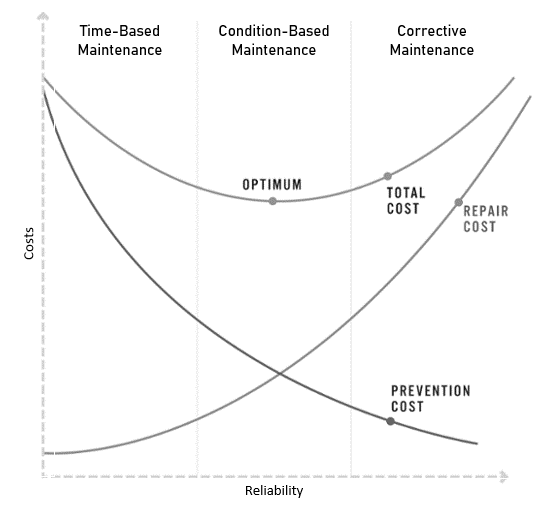
\includegraphics[scale=0.8]{Figures/optimummaintenance}
\caption[Comparison between TBM, CBM and CM]{Comparison between TBM, CBM and CM\footnotemark}
\label{fig:optimummaintenance}
\end{figure}
\footnotetext{https://www.losant.com/blog/using-iot-and-machine-learning-for-industrial-predictive-maintenance}

\subsection{Data cleaning} \label{Data cleaning}
By processing signals from sensors it may occur that a signal suffers unwanted modifications during capture, storage, transmission, or processing, called 'noise'. According to \citet{Ghasemi2010} also errors of measurements and interpretation due to limited accuracy of measurement instruments can cause noise. This noise have to be filtered because it limits the ultimate performances that can be obtained from a given device in terms of signals \parencite{BORDONI1990}. What type of noise occurs depends on the available sensors within a machine but mostly concern temperature, pressure, displacement, weak force, and voltage.

As mentioned before, noise should be eliminated from the equipment condition sensor measurements. In literature, various techniques are described that can separate this noise from actual sensor data. \citet{LESON2016} make use of a Gaussian noise filter, \citet{KALLEN2005} describe a Monte Carlo method and \citet{LU2013} a Quasi Monte Carlo method using the Genz transform to reduce the calculating time and obtain smaller errors. Furthermore, \citet{Bourdin2011} describes a non-local averaging method, that can be used in the frequency domain. Which method is chosen to eliminate the noise depends on the type of sensors that is used with their corresponding signal types. \\ \\
Other literature that might be handy to study extensively: 
\begin{itemize}
\item Probability distributions - books available at university library
\item Markov decision processes - books available at university library
\item Deterioration processes see \parencite{CHEN2015}, \parencite{Do2015}, \parencite{JARDINE2006}, \parencite{Sloan2000}
\end{itemize}
Study on these will only be done if the artifact that will be designed is actual dealing with those subjects. For this conceptual version of the project it is not interesting yet. 

\subsection{Implementing CBM} \label{Implementing CBM}
To implement CBM to an existing production process, several steps have to be taken. In Figure \ref{fig:Method CBM}, a method, based on \citet{maxgrip}, is depicted that shows these steps. Sensor data sets regarding robot arm conditions (temperatures, voltages, torques etc.) should be available from the RAC. This data sets will be matched with the Event logs, notes from mechanics about for example replacements and observed faults, in order to see what variables in the sensor data correspond with certain Event logs. From here, features/patterns should be detected by analyzing the data. \citet{Jaber2017} gives an overview of various techniques regarding vibrations, noise and Motor Current Signature Analysis (MCSA). Furthermore, \citet{Kahane2007} describes that some idea or hypothesis can be verified by gathering and analyzing data by means of regression analysis. One of these techniques should be applied to analyze relationships between variables. When features or patterns are detected by regression analysis or an other technique, a model can be constructed based on the analyzed relationships of variables. Thereafter, a techniques that can be used to train a model is necessary. A few techniques are described below briefly.
\begin{itemize}
\item \textbf{Fuzzy Logic} is a list of if-then statements, called rules, that can be used for computing with words rather than numbers. Although words are inherently less precise than numbers, their use is closer to human intuition \parencite{FuzzyToolbox}.
\item \textbf{Neuro-fuzzy} is a combination of fuzzy logic and neural networks. Fuzzy systems lack the ability to learn or adjust themselves. However, a system based on a neural network provides a promising approach for condition prediction models \parencite{Zhao2009}.  
\end{itemize}
\begin{figure}[ht]
\centering
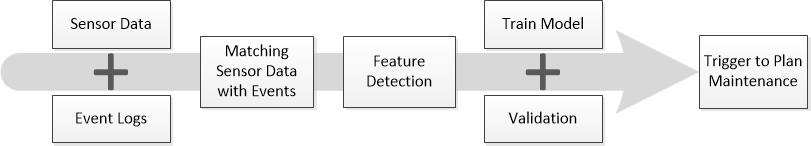
\includegraphics[width=\textwidth]{Figures/CBM_Method2}
\caption[Method of implementing CBM]{Method of implementing CBM}
\label{fig:Method CBM}
\end{figure}

In the ideal situation, CBM is able to detect problems so that equipment can be replaced or repaired before a failure. If the extra CBM related cost are less than or equal to other preventive replacement expenses, no corrective or time-based maintenance is needed \parencite{mckone2002}. However, as is described by \citet{ALNAJJAR20003}, CBM may not be 100\% accurate. It is possible that failure occurs before problems are predicted, and on other occasions, conditions will dictate equipment replacement and repair when the equipment could continue to operate for some time. If these prediction mistakes occurs frequently a combination with TBM should be developed where a trade-off between using TBM and CBM is considered.
% zeer handige site http://www-tandfonline-com.proxy-ub.rug.nl/action/doSearch?AllField=A+Failure+Time+Prediction+Method+for+Condition-Based+Maintenance Ook het artikel van Scarf 2007 is erg handig! Verder CTRL+F op scarf in de maintenance library, vrijwel alle artikelen van hem zijn aanraders!

\section{Conceptual Framework} \label{Conceptual Framework}
According to \citet{Wieringa2014}, when the goal is to design an artifact, it have to be ensured that the conceptual framework is understood by the users. The conceptual model for this project consist of three main constructs, Robot Assembly Cell, Maintenance Planning and Users, as is depicted in Figure \ref{fig:conceptual model}. Within every construct elements/functions/activities are defined and the relationships are represented by arrows. The design goal of this project focuses on applying a CBM tool to the Maintenance Decision Making process within the Maintenance Planning. Based on this description of the relations this process has with its environment, sub-questions are formulated in Section \ref{Sub-Questions}. A complete description of the conceptual model is given below:
\begin{figure}[ht]
\centering
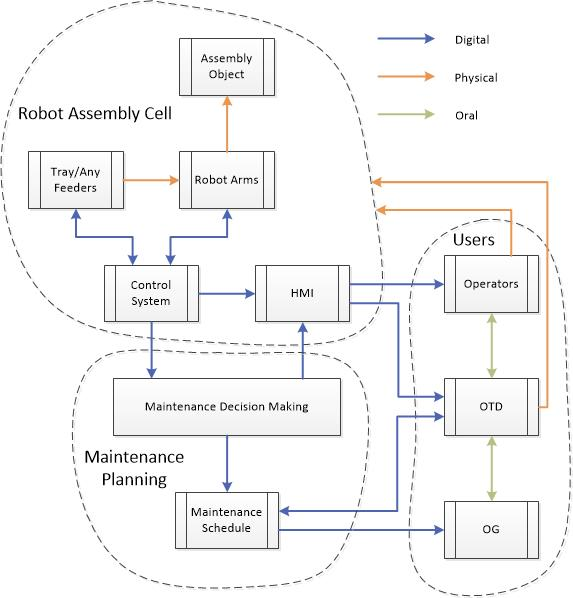
\includegraphics[width=\textwidth]{Figures/Conceptual_Model}
\caption[Conceptual model]{Conceptual model}
\label{fig:conceptual model}
\end{figure}

\begin{itemize}
\item The most important part in the conceptual model are the orange lines within the RAC, those activities determine the throughput of the RAC. Those lines between the \textbf{Tray/Any Feeders}, \textbf{Robot Arms} and \textbf{Assembly Object} correspond to the pick and place activities of the RAC, the assembly of holder and springs to the shaver unit. All other activities and streams within the conceptual model are in service of those physical activities. The Tray/Any Feeders require less maintenance than the Robot Arms and therefore only data available from the Robot Arms will be analyzed. 
\item The Tray/Any Feeders and Robot Arms are controlled by a \textbf{Control System}, installed on the RAC computer that assigns tasks. The systems (ACE, V+) that are used to control all RACs at Philips are described in Section \ref{RAC components}. Data from Tray/Any Feeders and Robot Arms (AC/DC Voltages, Temperatures, Torque, Position Errors and Duty Cycles among others) are transmitted to the Control System and are displayed by the Human Machine Interface (HMI). Furthermore, the same data is used to decide if maintenance is necessary and is therefore transmitted to the Maintenance Decision Making activity.
\item The \textbf{HMI} provides an interface so that the Operators and the OTD can interfere with the Control System of the RAC. As mentioned before, data available from Tray/Any Feeders and Robot Arms can be displayed at the HMI or extracted by connecting an external computer.
\item The \textbf{OTD} and \textbf{Operators} consult each other by operating and maintaining the RAC's (green line). The physical repair and maintenance is depicted by the orange lines connecting the OTD and Operators with the RAC. The OTD is responsible for maintenance at the RACs and the Operators are responsible for operating the entire ALs.
\item Consult takes also place between the OTD and the \textbf{OG}. Employees within those groups determine together if the RAC is working optimal or need maintenance. If maintenance is needed, the OTD provide this maintenance. Members of the OG are described in Section \ref{Stakeholder analysis}
\item This project focuses on designing the \textbf{Maintenance Decision Making} process. This process receives data from the Control System and should analyze this data so that it can predict if there is any upcoming maintenance. The output value of this process should than be a \textbf{Maintenance Schedule} that is constructed automatically for parts where maintenance is predictable. The OTD and OG can take action according to this Maintenance Schedule. Data analysis should also be displayed on the HMI so that it can be seen what values determined that maintenance should be planned.
\end{itemize} 

\section{Sub-Questions} \label{Sub-Questions}
In order to contribute to the research goal of this project, an artifact have to be designed and sub-research questions can be formulated. In Section \ref{Comparison of TBM and CBM} is concluded that CBM has the highest potential in decreasing maintenance cost. Therefore, sub-questions regarding a CBM tool can be formulated. Furthermore, in Section \ref{Conceptual Framework} it can be seen what elements and relations play a role by improving the maintenance schedule. The sub-questions will be based on the conceptual model regarding these relations. The following questions are formulated with respect to the question constraints described by \citet{Wieringa2014}. \\ \\ 
Sub-question 1:
\begin{center}
\textit{What data types, available from the control system, can predict maintenance activities?}
\end{center}
To design a predictive maintenance tool, data that is able to predict upcoming maintenance should be analyzed. Answering this empirical knowledge question will result in a description of the relationship between data and the maintenance it might predict. \\ \\
Sub-question 2:
\begin{center}
\textit{How can the output data be interpret in order to predict maintenance?}
\end{center}
From question 1 it is determined what data types are relevant by predicting maintenance. It is necessary to investigate how this data should be interpreted in order to make realistic estimations. In other words, answering question 2 result in a designed artifact that can predict upcoming maintenance. \\ \\
Sub-question 3:
\begin{center}
\textit{On what performance indicators should the artifact be evaluated?}
\end{center}
After an artifact is designed, its performance have to be tested and evaluated in order to validate the design. If the artifact is evaluated successful, it have to supply the maintenance schedule.\\ \\
Sub-question 4:
\begin{center}
\textit{What are requirements for software engineers to integrate the artifact in the control system?}
\end{center}
After designing an artifact, software engineers from Beenen have to integrate it into the HMI of the RACs. During the design phase, requirements for this integration should be considered.



\chapter{Experimental Setup} \label{Chapter4}

\section{RAC components} \label{RAC components}
In order to provide a solution to the goals stated in Section \ref{Business context} it is important to obtain a good understanding of all aspects that play a role within the RAC. A short description of all hardware and software aspects is given below. It is possible that not all described components are relevant to this project. Nevertheless, some terms may be used throughout this thesis and therefore a brief description of these components can be helpful. Section \ref{Hardware} gives an overview of the hardware components within the RAC, the robotic arm, vision camera and any feeder. The robotic arm will be discussed more thoroughly because that aspect requires the most maintenance and is therefore more interesting. Section \ref{Software} gives an overview of all software components within the RAC, V+\textsuperscript{\tiny{TM}}, ACE\textsuperscript{\tiny{TM}}, and AdeptSight\textsuperscript{\tiny{TM}} that play a role by designing the CBM tool.

\subsection{Hardware} \label{Hardware}
As mentioned before, the RAC consist of several components (anyfeeder, vision camera, robotic arm, conveyor belt). The vision cameras and the robotic arms are products of Bremer Werk für Montagesysteme (BWM), a company that produces assembly systems, automation systems, and special-purpose machine manufacturing\footnote{https://www.bwm-gmbh.de/en/unternehmen/}. BWM has established the ALs at Philips by installing the RACs and providing controllers to the components. For example, the trajectory that a robotic arm has to execute in order to assemble certain parts of a shave is programmed by BWM. 

The vision guidance system and Adept AnyFeeder\textsuperscript{\tiny{TM}} that are part of RB34 are not discussed in detail. Obtaining data from the anyfeeder is a complex task that should be performed by Adept programmers and will be outside the scope of this project. Maintenance on the vision guidance system is rare and therefore it is not relevant to predict it.  

The robotic arms within RAC RB34 that are used to assemble the shaver units are Adept Cobra s600's with four axis. This is a high-performance Selective Compliance Assembly Robot Arm (SCARA) robot system for mechanical assembly, material handling, packaging, machine tending, screw driving, and other applications that require fast and precise automation. This robot include the Adept SmartController EX\textsuperscript{\tiny{TM}} motion controller, an ultra-compact, high-performance, distributed robot motion controller capable of controlling an entire production line managing multiple robots. Before this project, RB34 featured a Smart Controller CX\textsuperscript{\tiny{TM}} which is not able to subtract the data from the RAC due to complex programming issues. Therefore, Smart Controller EX, a newer version motion controller from adept, is installed on RB34 especially for this project. In Figure \ref{fig:Cobra s600} and \ref{fig:SmartController} the robot arm and the motion controller are depicted, respectively, and a full description of the hardware is available on the website of Adept\footnote{http://www.adept.com/products/robots}.
\begin{figure}[ht]
\centering
\begin{subfigure}[b]{0.49\textwidth}
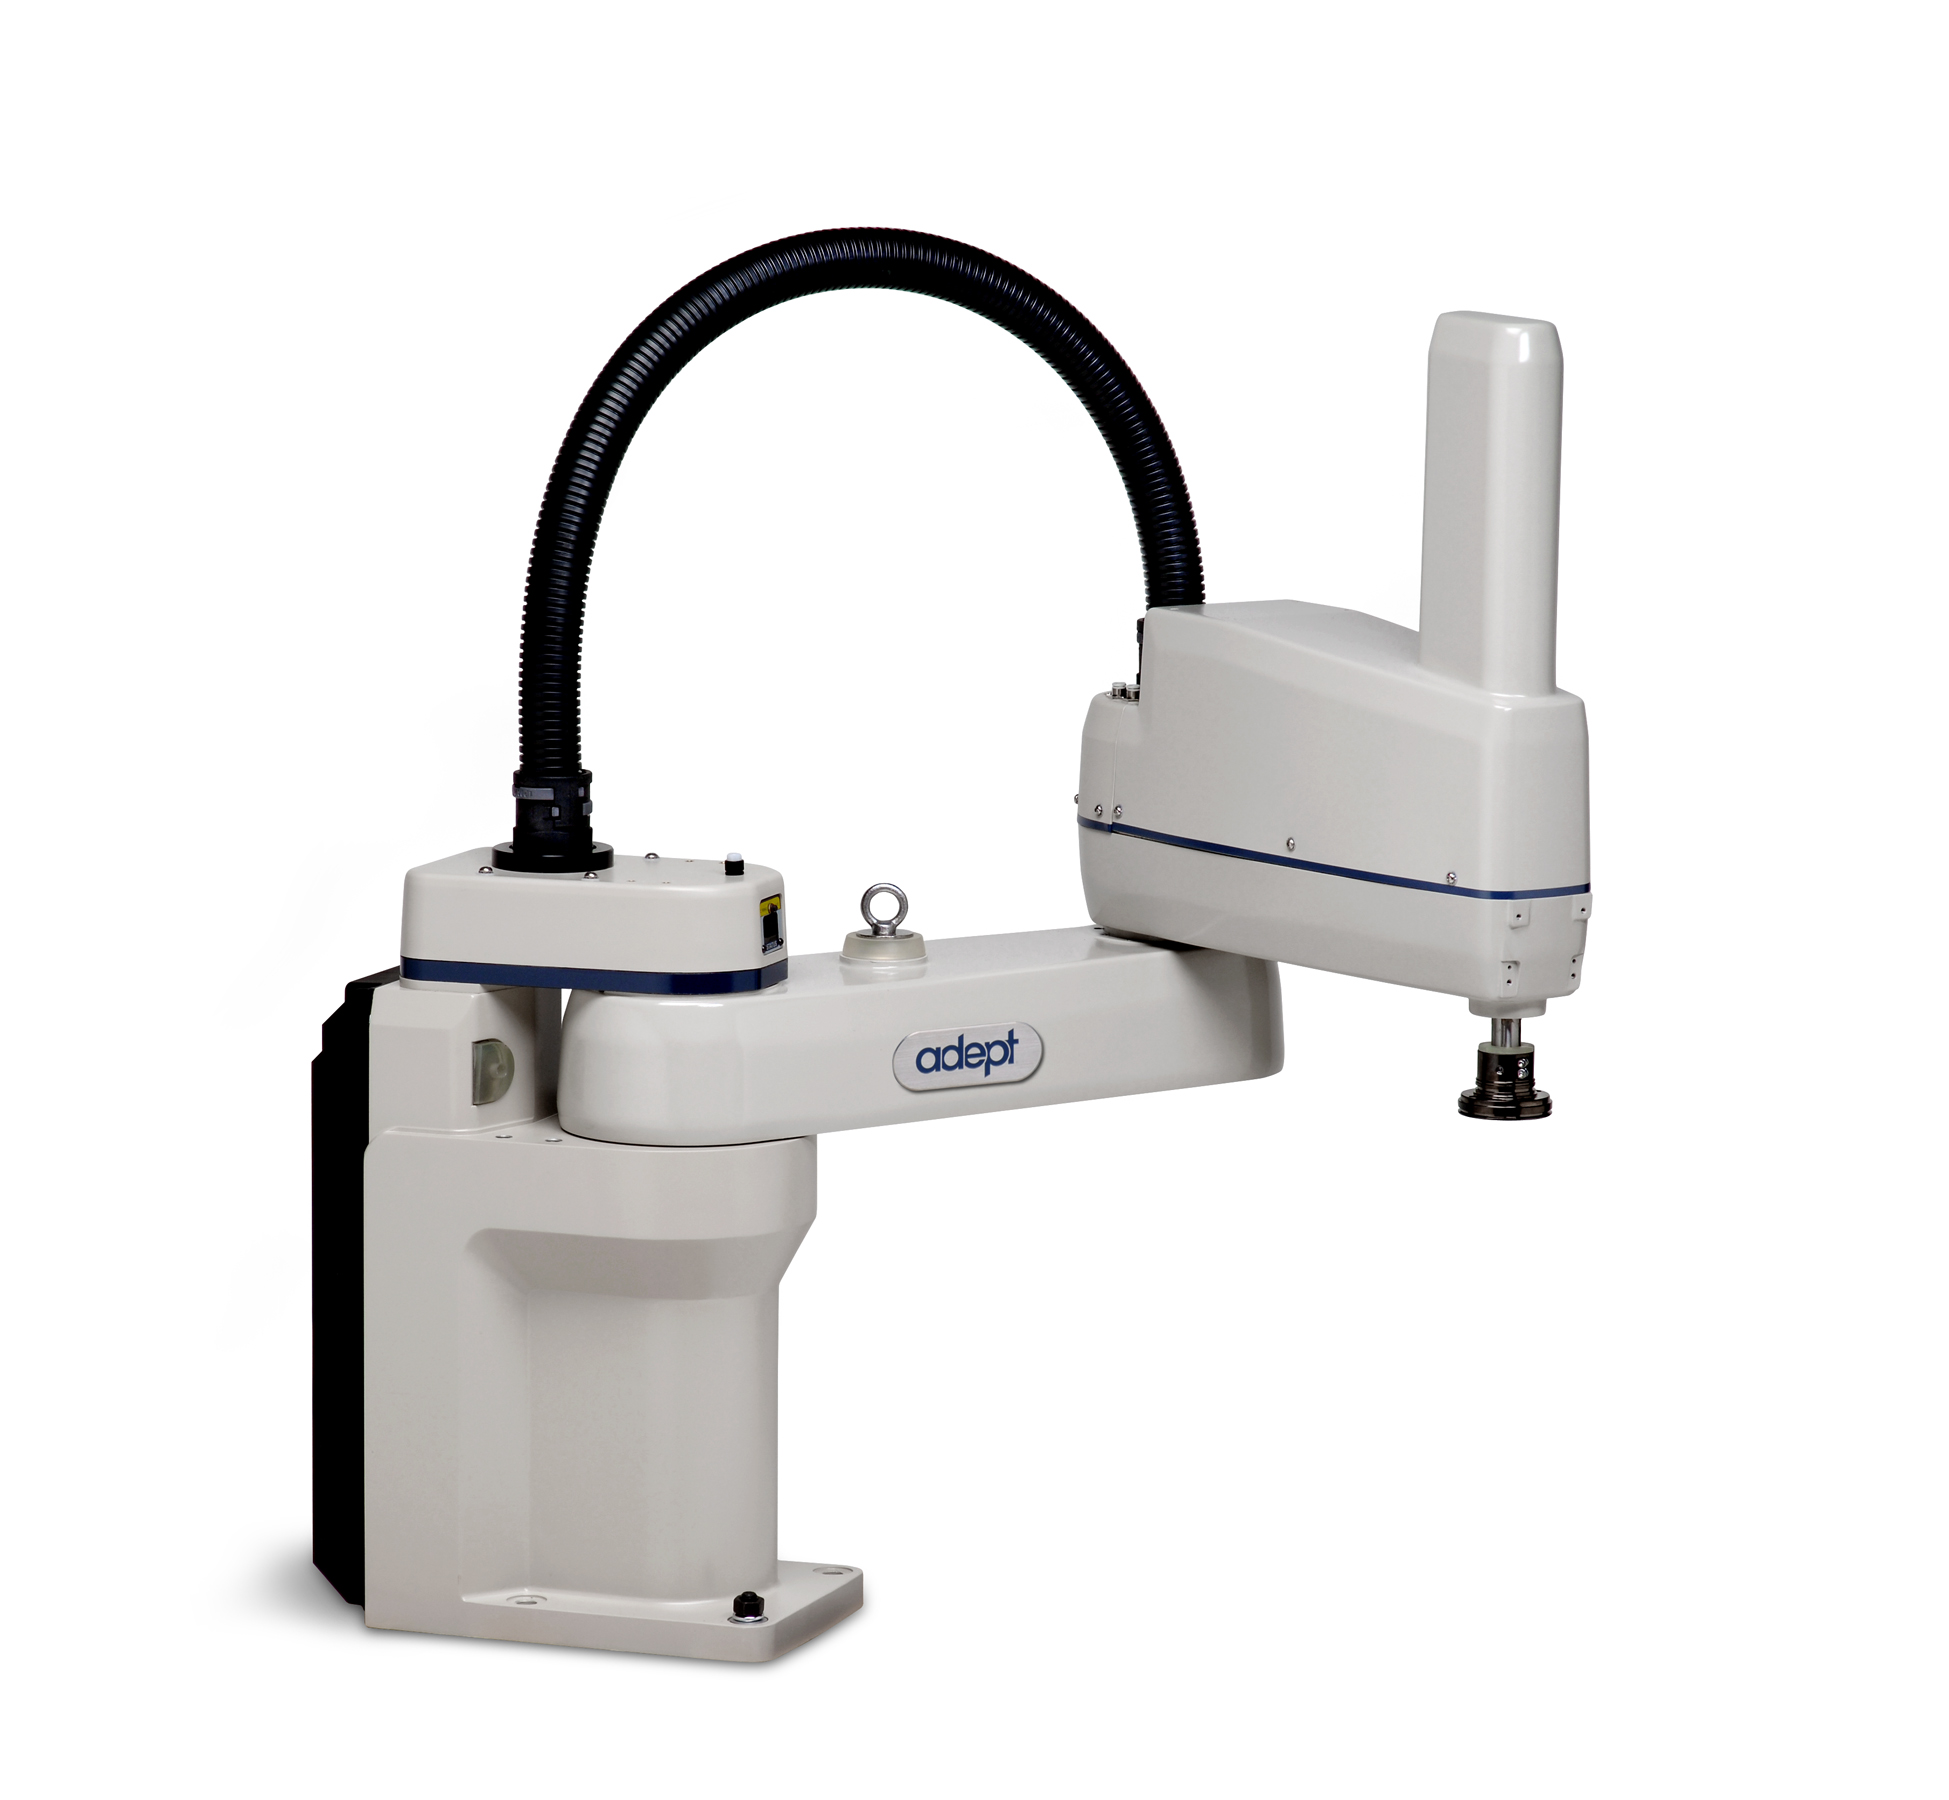
\includegraphics[width=\textwidth]{Figures/Cobra-600}
\caption{Adept Cobra s600}
\label{fig:Cobra s600}
\end{subfigure}
\begin{subfigure}[b]{0.49\textwidth}
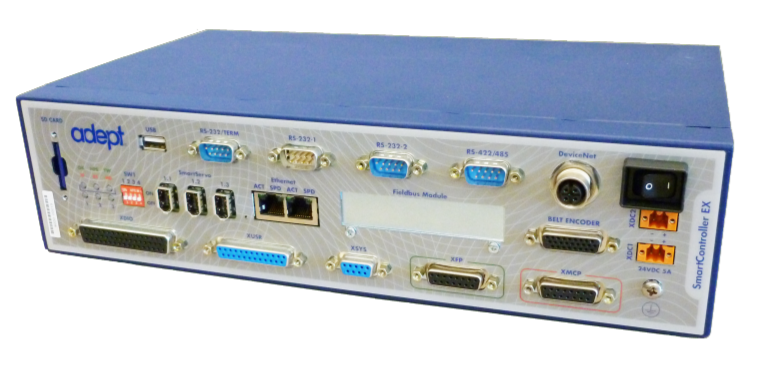
\includegraphics[width=\textwidth]{Figures/SmartController}
\caption{Adept SmartController EX}
\label{fig:SmartController}
\end{subfigure}
\caption[Relevant hardware components of RB34]{Hardware components of RB34}
\label{fig:HardwareComponents}
\end{figure}

\subsection{Software} \label{Software}
The programming language that is used is V+, a language to provide an integrated solution to all of the programming needs in a robotic workcell, including safety, robot motion, vision operations, force sensing and I/O. It is used to combine the vision guidance software with the control software that is installed on the PC of the RAC. 

AdeptSight\textsuperscript{\tiny{TM}} is an easy-to-use, standalone vision guidance and inspection package and comes complete with all the necessary accessories. The software includes a powerful framework that can be used to develop customized vision guidance and inspection applications. 

The interaction with operators at the RACs is provided by an interface called ACE (Automation Control Environment) which features an integrated environment for robot and control. Data is available for every robotic arm motor regarding temperature, torque, voltage, position error and duty cycle and can be displayed on the Human Machine Interface (HMI) which is connected with the control system of a RAC. The different types of data and their relevance are discussed in Section \ref{Data Gathering}.

\section{Data gathering} \label{Data Gathering}
In this section, data that is useful for the execution of the research will be presented. By analyzing the useful data, the relevant data to investigate can be determined research question one will be answered and research question one will be answered. Data that can be subtracted from the RAC controller is mentioned briefly. In table \ref{Data types}, all data types that can be obtained are listed. From those types of data it should be determined which type is relevant and is able to predict  maintenance. Since all Cobra s600  robots within the AL are identical and execute similar tasks, it is assumed that the same data type(s) will predict similar maintenance for all Cobra s600 robots. 

%A new table should be build to list all data types. The data types are available on http://www1.adept.com/main/ke/data/pdf_web/ace_ug.pdf. 
%\begin{table}[ht]
%\centering
%\caption[Data types available from the SmartController]{Data types available from the SmartController}
%\label{Data types}
%\begin{tabular}{l | l | l}
%\multicolumn{3}{|c|}{Data Type} \\
%\hline
%Robot Bus Voltage & Voltage \\
%Robot AC input & Root-mean-square (RMS) Voltage \\
%Robot DC input & Voltage \\
%Robot Base board temperature & $^\circ$Celsius \\
%Motor Amplifier temperature & $^\circ$Celsius \\
%Motor Duty cycle & \% limit \\
%Motor Peak torque & \% maximum torque \\
%Motor Peak velocity & Revolutions per Minute (RPM) \\
%Motor Peak position error & \% soft envelope error
%\end{tabular}
%\end{table}

\begin{table}[ht]
\centering
\caption[Data types available from the SmartController]{Data types available from the SmartController}
\label{Data types}
\begin{tabular}{l | c}
Data type & Unit \\
\hline
Robot Bus Voltage & Voltage \\
Robot AC input & Root-mean-square (RMS) Voltage \\
Robot DC input & Voltage \\
Robot Base Board temperature & $^\circ$Celsius \\
Motor Amplifier temperature & $^\circ$Celsius \\
Motor Duty cycle & \% limit \\
Motor Peak torque & \% maximum torque \\
Motor Peak velocity & Revolutions per Minute (RPM) \\
Motor Peak position error & \% soft envelope error 
\end{tabular}
\end{table}

\begin{figure}[ht]
\begin{subfigure}{.5\textwidth}
 \centering
 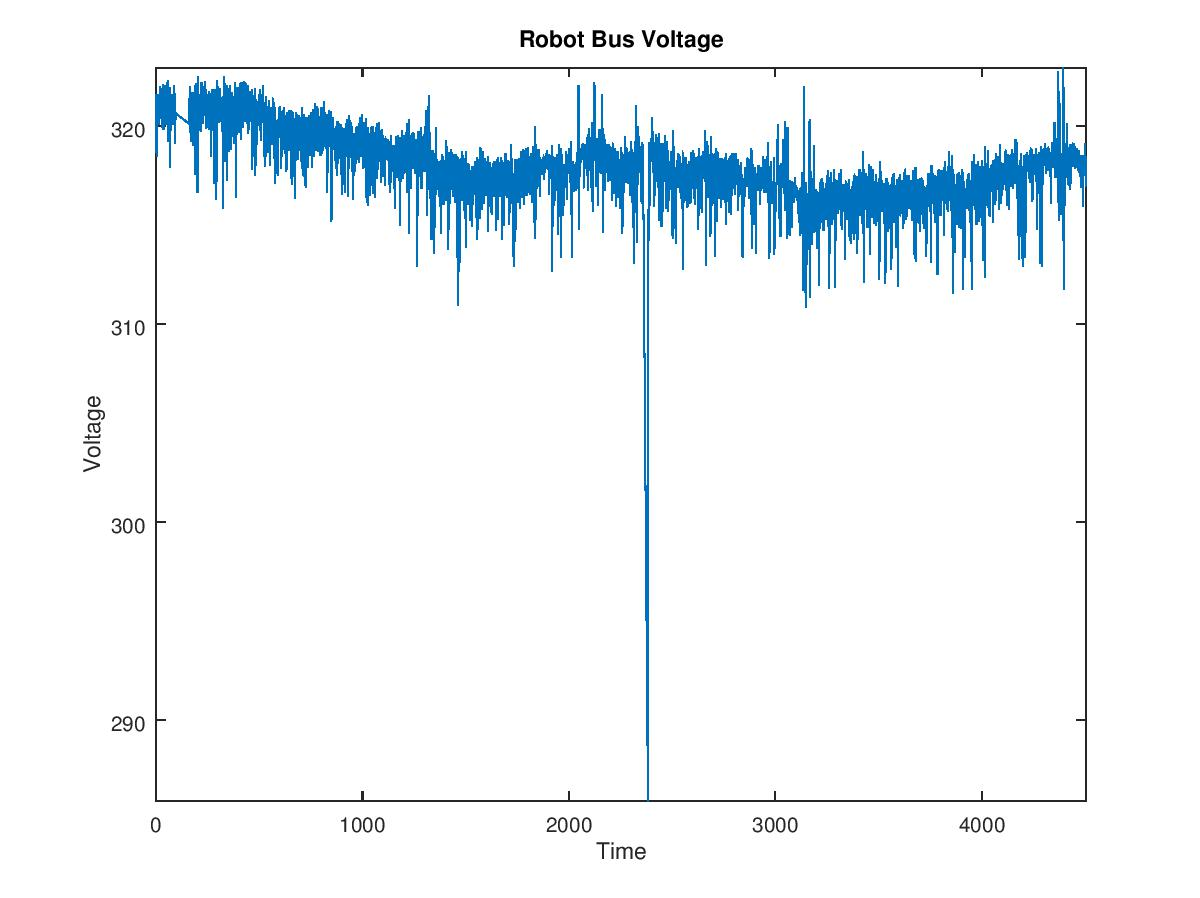
\includegraphics[width=.9\linewidth]{Figures/Robot_Bus_Voltage}
 \caption{Robot Bus Voltage}
 \label{fig:Robot Bus Voltage}
\end{subfigure}
\begin{subfigure}{.5\textwidth}
 \centering
 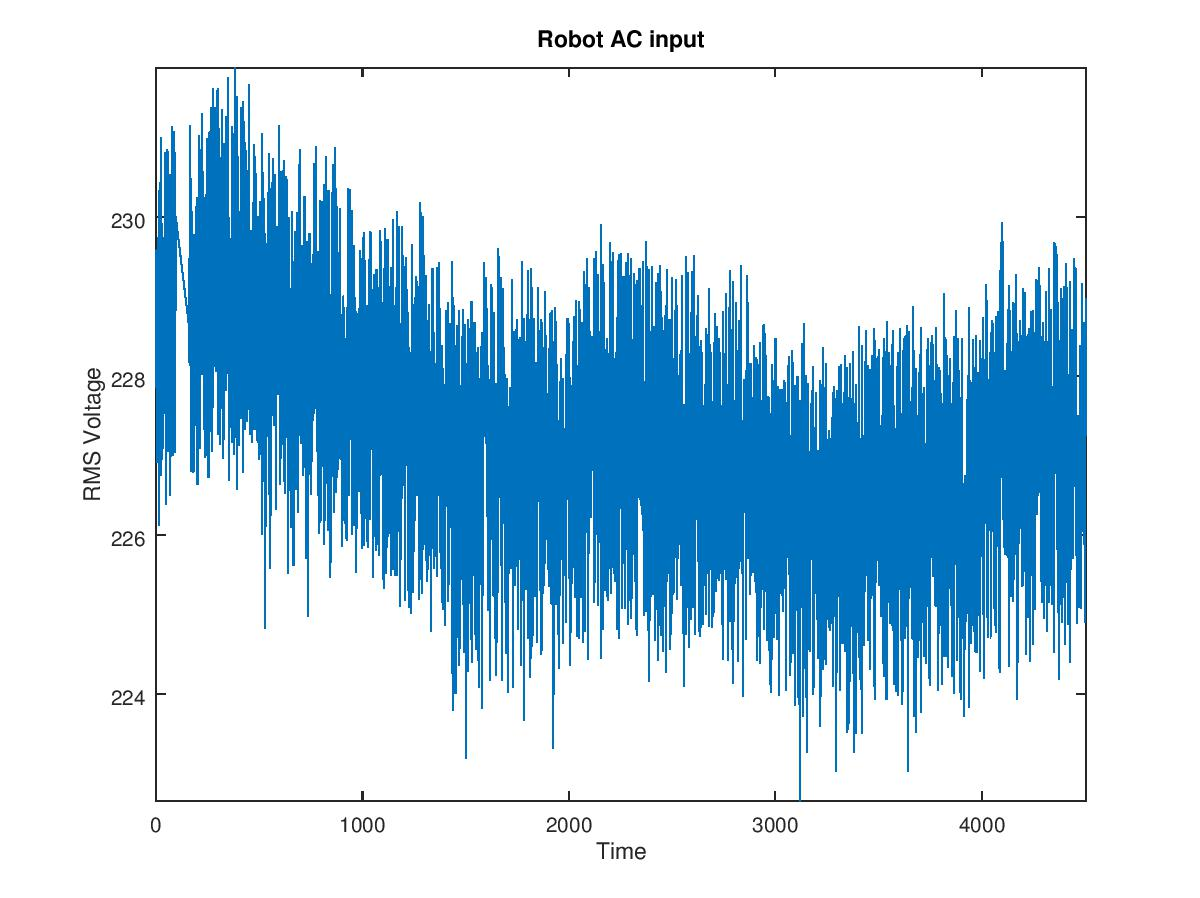
\includegraphics[width=0.9\linewidth]{Figures/Robot_AC_input}
 \caption{Robot AC input}
 \label{fig:Robot AC input}
\end{subfigure}\\
\begin{subfigure}{.5\textwidth}
 \centering
 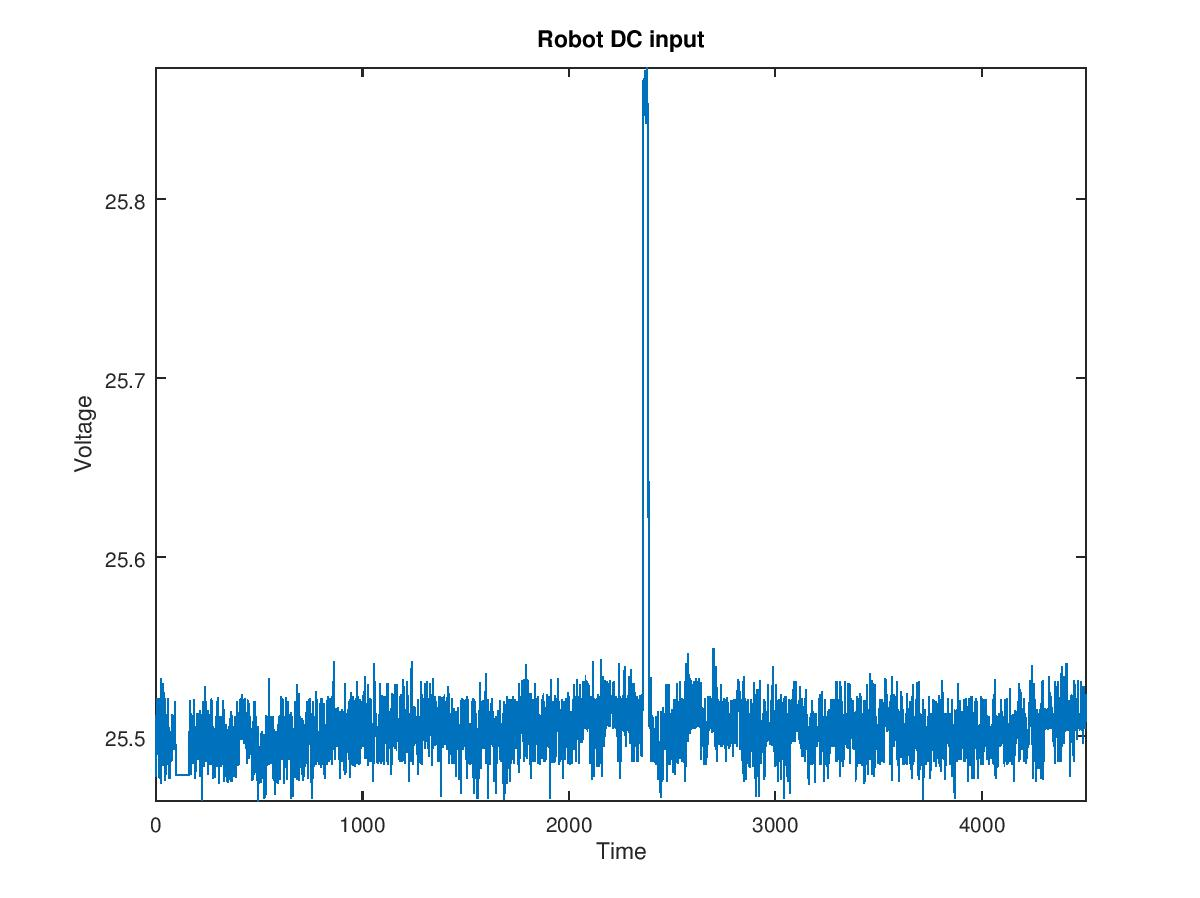
\includegraphics[width=.9\linewidth]{Figures/Robot_DC_input}
 \caption{Robot DC input}
 \label{fig:Robot DC input}
\end{subfigure}
\begin{subfigure}{.5\textwidth}
 \centering
 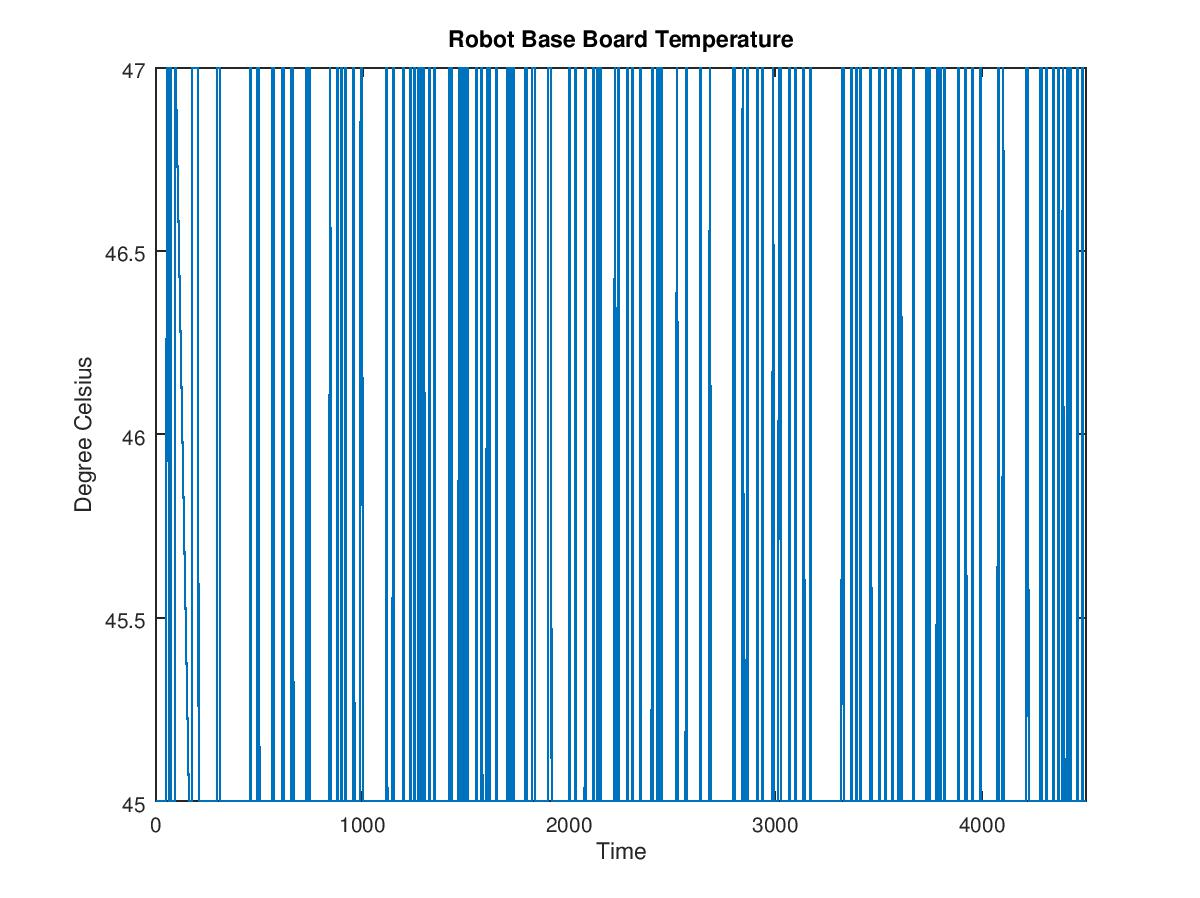
\includegraphics[width=.9\linewidth]{Figures/Robot_Base_Board_Temperature}
 \caption{Robot Base Board Temperature}
 \label{fig:Robot Base Board Temperature}
\end{subfigure}\\
\begin{subfigure}{.5\textwidth}
 \centering
 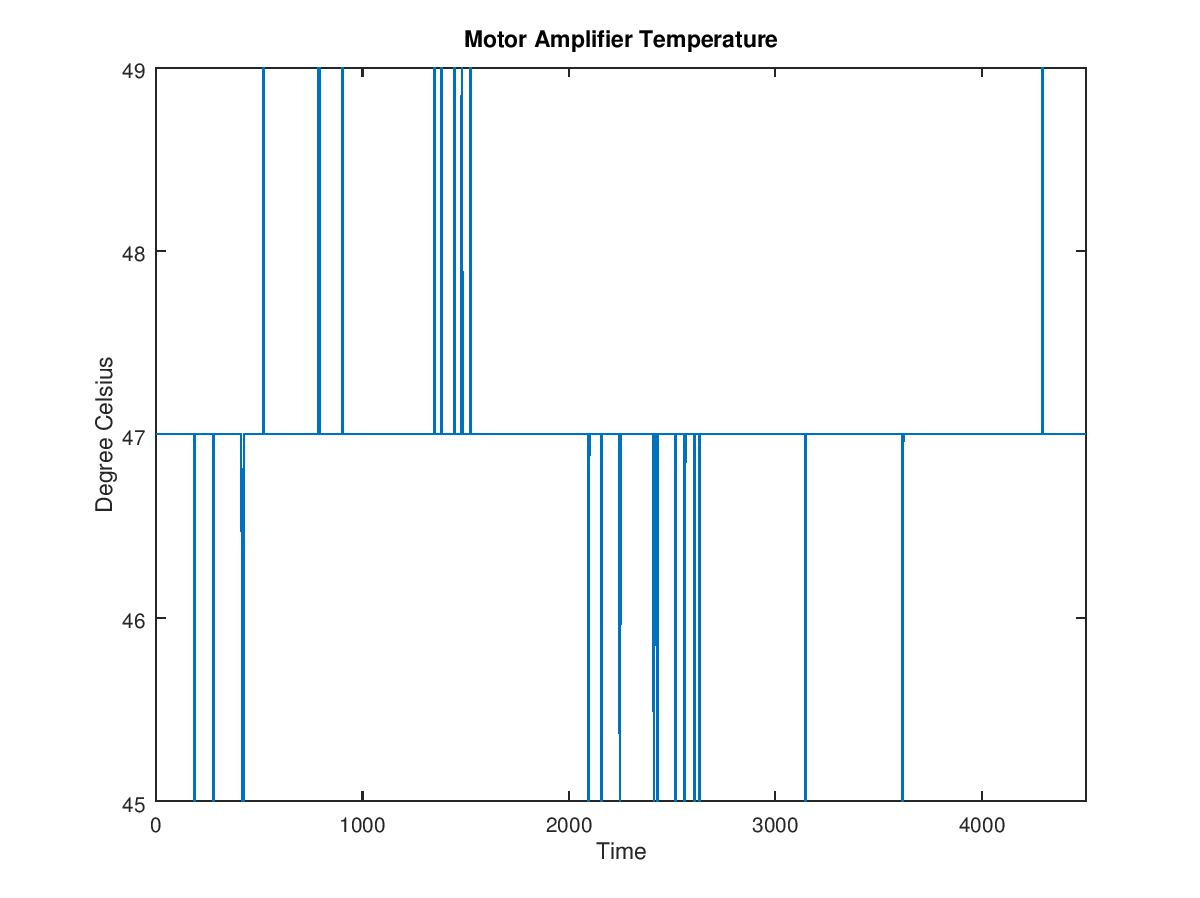
\includegraphics[width=.9\linewidth]{Figures/Motor_Amplifier_Temperature}
 \caption{Motor Amplifier Temperature}
 \label{fig:Motor Amplifier Temperature}
\end{subfigure}
\begin{subfigure}{.5\textwidth}
 \centering
 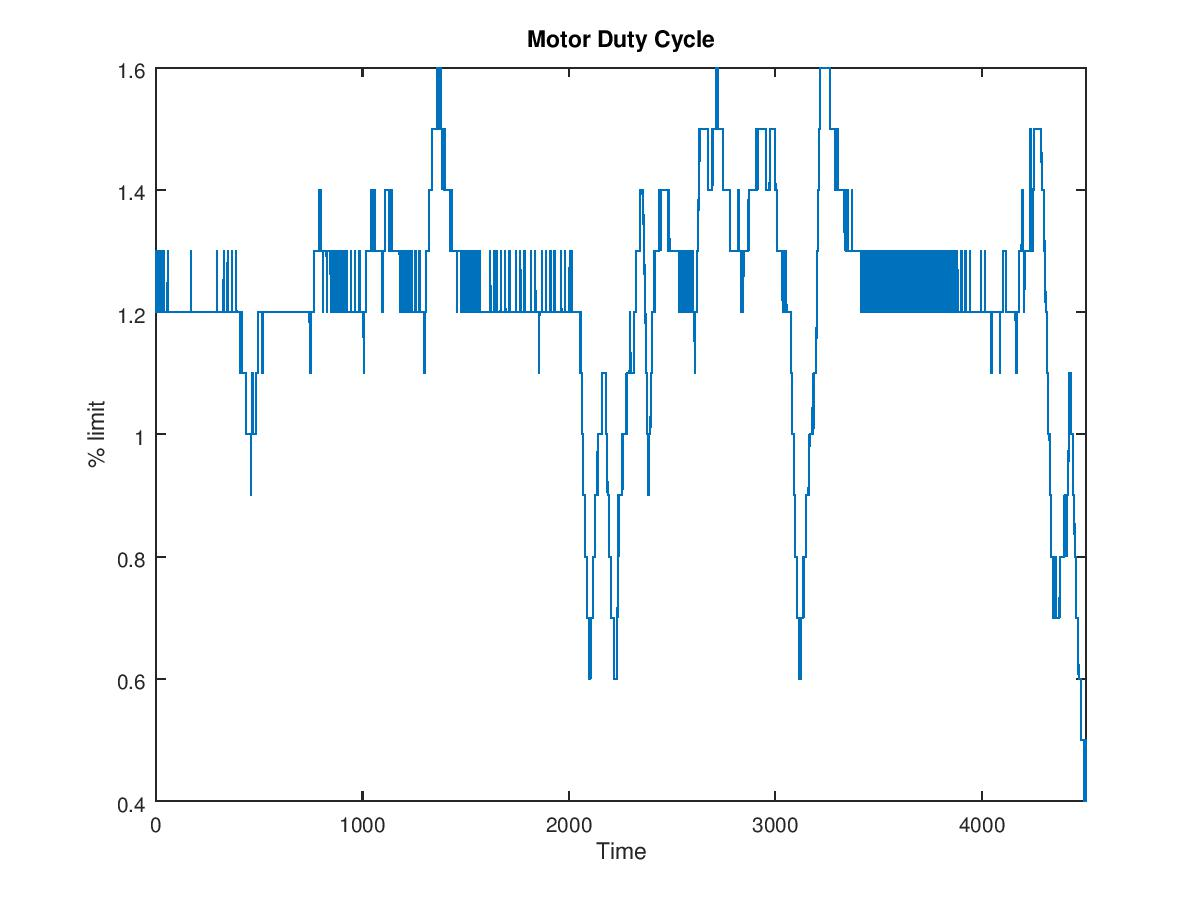
\includegraphics[width=.9\linewidth]{Figures/Motor_Duty_Cycle}
 \caption{Motor Duty cycle}
 \label{fig:Motor Duty Cycle}
\end{subfigure}
\caption[Data type plots]{Data type plots}
\label{fig:Data types}
\end{figure}

\subsubsection{Robot Bus Voltage}
\subsubsection{Robot AC input}
\subsubsection{Robot DC input}
\subsubsection{Robot Base board temperature}
\subsubsection{Motor Amplifier temperature}
\subsubsection{Motor Duty cycle}
\subsubsection{Motor Peak torque}
\subsubsection{Motor Peak velocity}
\subsubsection{Motor Peak position error}

\chapter{Data Analysis} \label{Chapter5}

\section{SQ1: What data types, available from the control system, can predict maintenance activities?} \label{SQ1}
How the different types of data can be extracted from the RAC's is explained in Section \ref{Data Gathering}. For every type of data that can be collected, it have to be determined if it is able to predict failures and therefore upcoming maintenance. Firstly, to understand what type of data should be collected and analyzed, it have to be determined which components from a robot arm require most costly maintenance. Cheap components or components that are easy to replace will not be considered since there is little to gain. Therefore, the CBM tool should focus at components that are costly or time-consuming to maintain and repair. From interviews with OTD employees and the Maintenance Engineer it is determined that the components within a robot arm joint are most time-consuming and costly to repair or replace. Therefore, this research will focus on these type of maintenance activities. Secondly, it have to be determined what data types are able to predict abnormality in robot arms and can be used to provide robot condition estimations. 

\subsection{Failure modes} \label{Failure modes}
In the maintenance logbook from Philips, all maintenance activities/event logs from 2011 to present are listed. In Figure \ref{fig:Cobra joint failures} it can be seen how many failures and events are related to which joint of a robot arm. Only the failures regarding Cobra s600s and s800s are included since those arms are similar and used mostly. In total, 97 major robot arm joint failures occurred and replacement was necessary. The number of failures per joint are 22, 64, 6, and 3 for joints 1, 2, 3, and 4, respectively. This is depicted in Figure \ref{fig:Cobra joint failures}. For most robot arms at Philips joint 1 and 2 are the joints with the highest average speed and torque and therefore it is assumed that joints with high speed and torque are more likely to fail. For this reason, data available from the joint of a robot arm with the highest average speed and torque will be focused on. 

Furthermore, the maintenance logbook shows that most failures are related to harmonic drive and motor failure. In total, 110 components were replaced where the motor and the harmonic drive caused failure mostly. The number of replaced components is higher than the number of failures since some failures required maintenance on multiple components. The number of failures per joint component is depicted in Figure \ref{fig:Joint failure component}. According to mechanics at Philips, motors and harmonic drives are replaced simultaneously and failure of a harmonic drive is the reason that a motor fails. Oil from a broken harmonic drive leaks through the motor and causes it to fail. 
\begin{figure}[ht]
\begin{subfigure}{.5\textwidth}
\centering
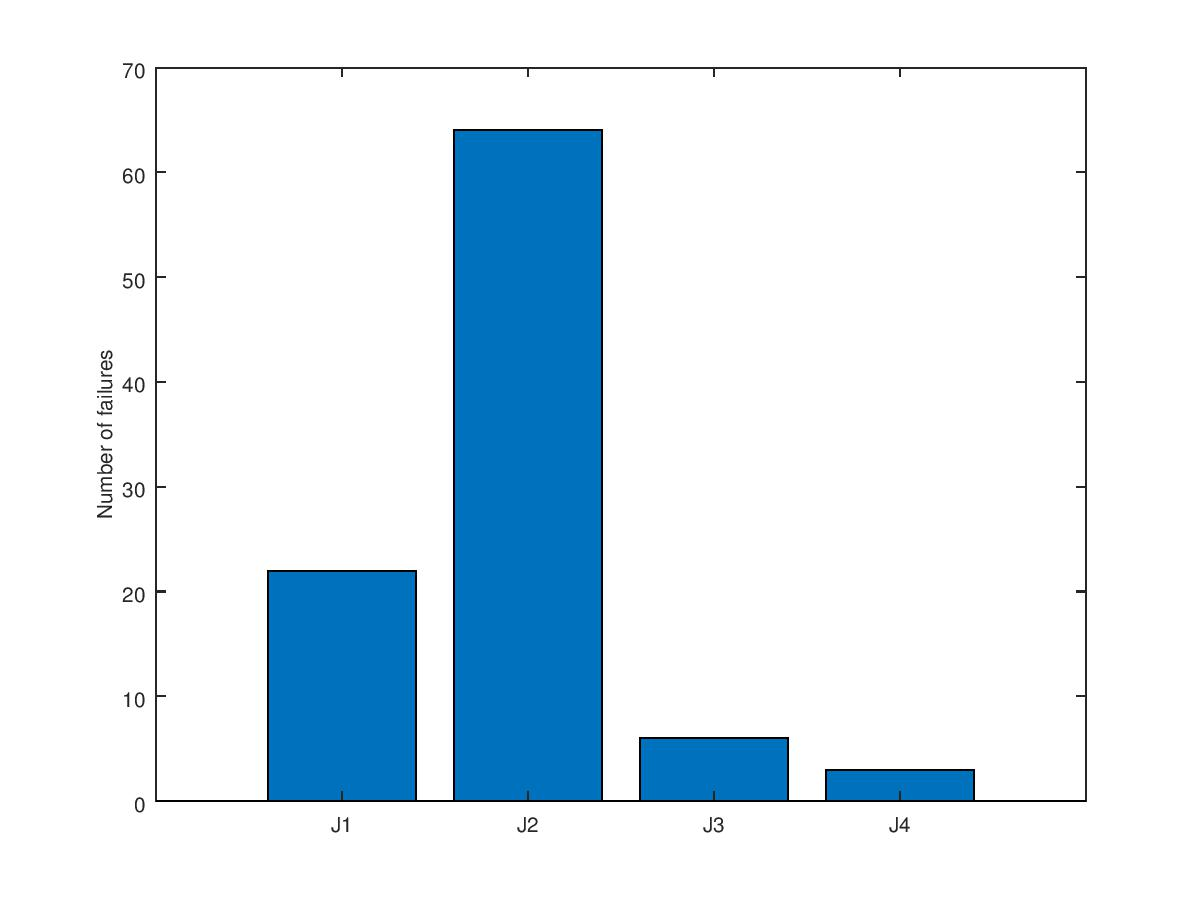
\includegraphics[width=.9\linewidth]{Figures/Cobra_joint_failures}
\caption[Number of Cobra s600/s800 joint failures]{Number of Cobra s600/s800 joint failures}
\label{fig:Cobra joint failures}
\end{subfigure}
\begin{subfigure}{.5\textwidth}
\centering
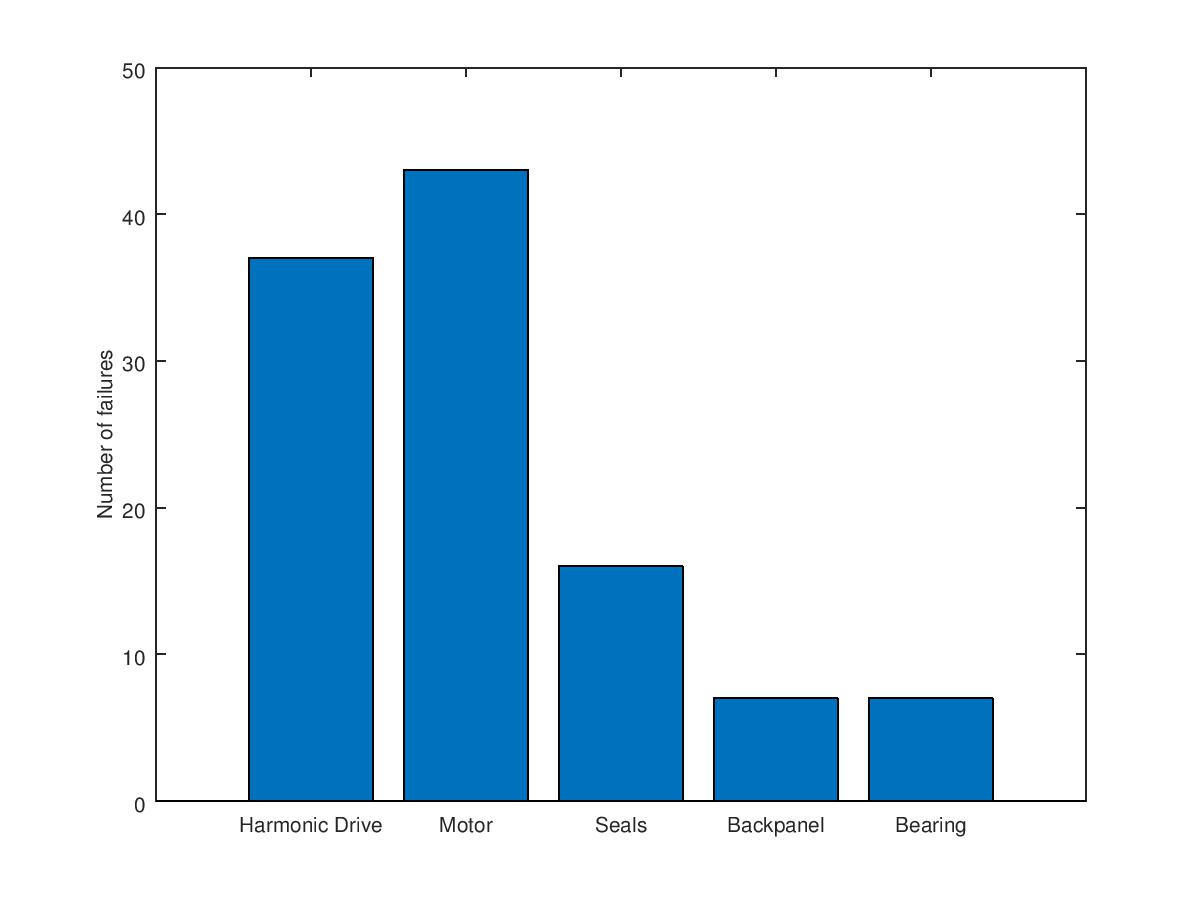
\includegraphics[width=.9\linewidth]{Figures/Joint_failure_component}
\caption[Number of failures per joint component]{Number of failures per joint component}
\label{fig:Joint failure component}
\end{subfigure}
\caption[Failure modes]{Robot arm failure modes. ({\tiny{A}}) Shows the number of failures that occurred at corresponding joints. ({\tiny{B}}) shows the components within a joint where a failure occurred.}
\label{fig:Failure data}
\end{figure}
As described in Section \ref{Hardware}, the harmonic drive of a Cobra s600 is exposed to wear and fatigue elements due to friction within the components. If the friction within a harmonic drive can be determined, an estimation of the component condition can be given and a RUL can be estimated. Friction is dependent on the contact geometry, topology, properties of the materials, relative velocity, lubricant, etc. \parencite{Al-Bender2008}. According to \citet{Bittencourt2012}, the following factors will be more or less significant to the total friction:
\begin{multicols}{2}
\begin{itemize}
\item temperature,
\item force/torque levels,
\item position,
\item velocity,
\item acceleration,
\item lubricant properties.
\end{itemize}
\end{multicols} 

\subsection{Relevant data} \label{Relevant data}
Based on the statements from the previous section, data available from the data collection methods, described in Section \ref{Data Gathering}, will be investigated on their relevance. According to the Adept User's Guide, force/torque levels are proportional to DC input voltages. Furthermore, the position error of a joint, the difference between the commanded position and the actual position, can be used to determine robot arm accuracy. As mentioned before, lubricant properties and temperature can also indicate robot failure. However, it is difficult to analyze lubricant continuously and will therefore not be investigated.

\subsubsection{DC Input Voltage} \label{DC Input Voltage}
The electric motor drives use power transistors to deliver energy. These transistors produce voltage; current is generated by the electrical circuit that is formed from the drive voltage and the motor windings. Because the power transistors produce voltage, a current loop is required to achieve precise control of current. A current loop compares the current command to the feedback and adjusts the drive voltage to minimize the error. 

\citet{Rajagopalan2006} proved theoretically and validated experimentally that faults in gears coupled to electric motors can be detected by monitoring either the voltage or the current in the motor driving the gear. Within their experiments they tested three types of gear faults: i) damaged gear tooth (local-tooth fault - deformation in one or two teeth), ii) scoring (loss of lubrication), and iii) debris in lubricant. They further describe that abnormality in an electric motor should appear in the stator voltage because a current-controlled motor should have no-stator-current harmonics as the motor current is regulated to the reference value. This indicates that when a motor of a Cobra s600 shows abnormality in voltage, it is related to abnormality in the applied torque. Data collection from a new assembly line, with the Adept ACE software, showed that the the voltage and current applied to the amplifier are oscillating around certain values. During motion, the DC input voltage is changing according to the commanded position. This can be seen in Figure \ref{fig:Electric Values}, where the commanded position and the corresponding voltage are depicted from a Cobra s600 during operation. When a negative position is required, the input voltage decreases and when a positive position is required, the input voltage increases. As mentioned above, abnormality in the input voltage is related to abnormality in applied torque. This indicates that analyzing DC input voltage can be used to predict abnormal behavior of a robot arm. However, the data is collected by the Data Collection Tool, as described in Section \ref{Data Gathering}, with a frequency of 1000 Hz. This function is not available on assembly lines with the Adept Desktop software and hence, other types of data will be analyzed so that a model can be designed which is useful for Adept ACE and Adept Desktop software. 
\begin{figure}[ht]
\centering
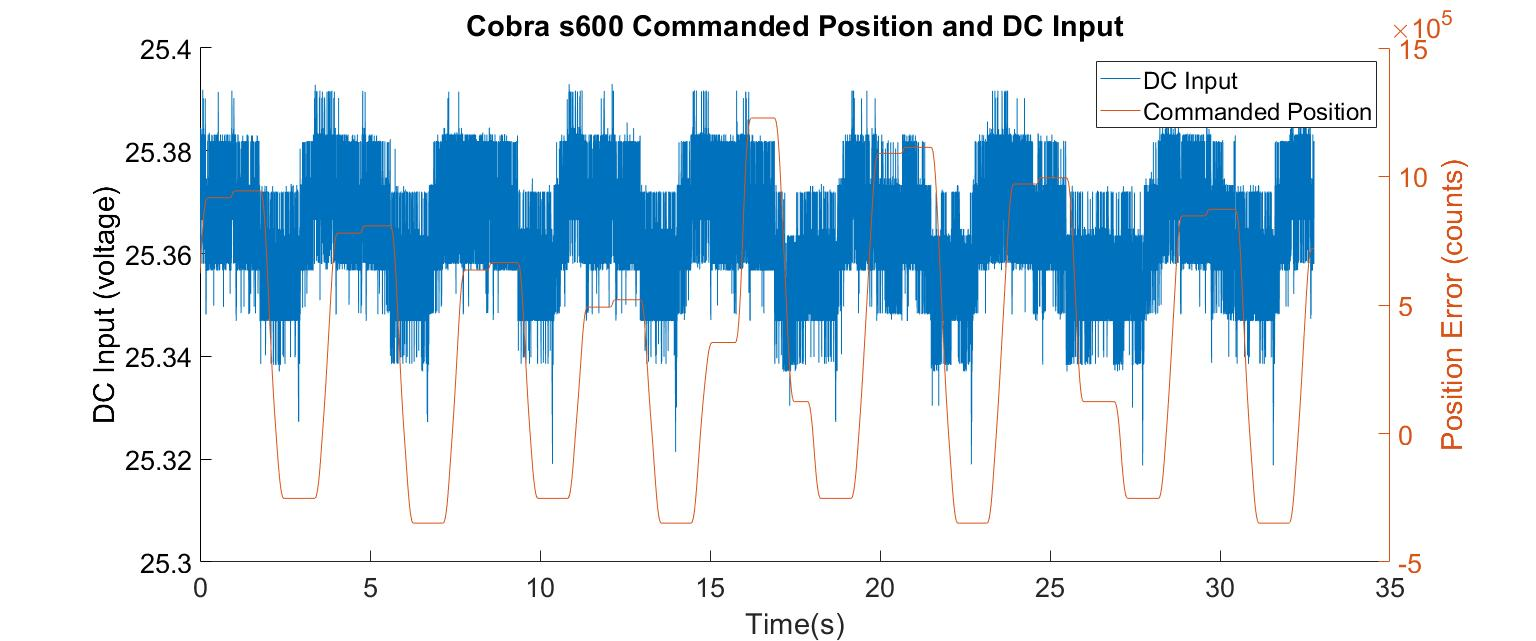
\includegraphics[width=\textwidth]{Figures/ComPosDCIn20}
\caption[DC Input voltage and Commanded Position for Cobra s600]{DC Input voltage and Commanded Position for Cobra s600} \label{fig:Electric Values}
\end{figure}

\subsubsection{Temperature} \label{Temperature}
As mentioned in Section \ref{Failure modes}, a changing temperature of a motor can also indicate failure. The robot arm joint motors are not equipped with temperature sensors. However, the encoder, located inside the robot arm joint motors, is equipped with a temperature sensor. When the temperature of a motor increases, the temperature of the encoder will increase as well.

To investigate if the encoder temperature can indicate robot joint failure, the daily average encoder temperatures from faulty and normal operating robot joints are reviewed. In Figure \ref{fig:AvgEncTemp}, it can be seen that faulty robot joints have, on average, a higher encoder temperature. This can indicate that the temperature of the corresponding motor is higher at faulty robot joints than normal operating joints. However, there are other causes that explain encoder temperature differences. The encoder can translate the robot joint position to the controller and does this by measuring the traveled distance of a joint motor. When this distance is large and/or the speed is high, the temperature of the encoder is increased. This indicates that a high encoder temperature is not only related to the motor temperature but also to the traveled distance and speed. To research whether the encoder temperature can indicate motor failure, monitoring the temperature values will be continued daily. 
\begin{figure}[ht]
\centering
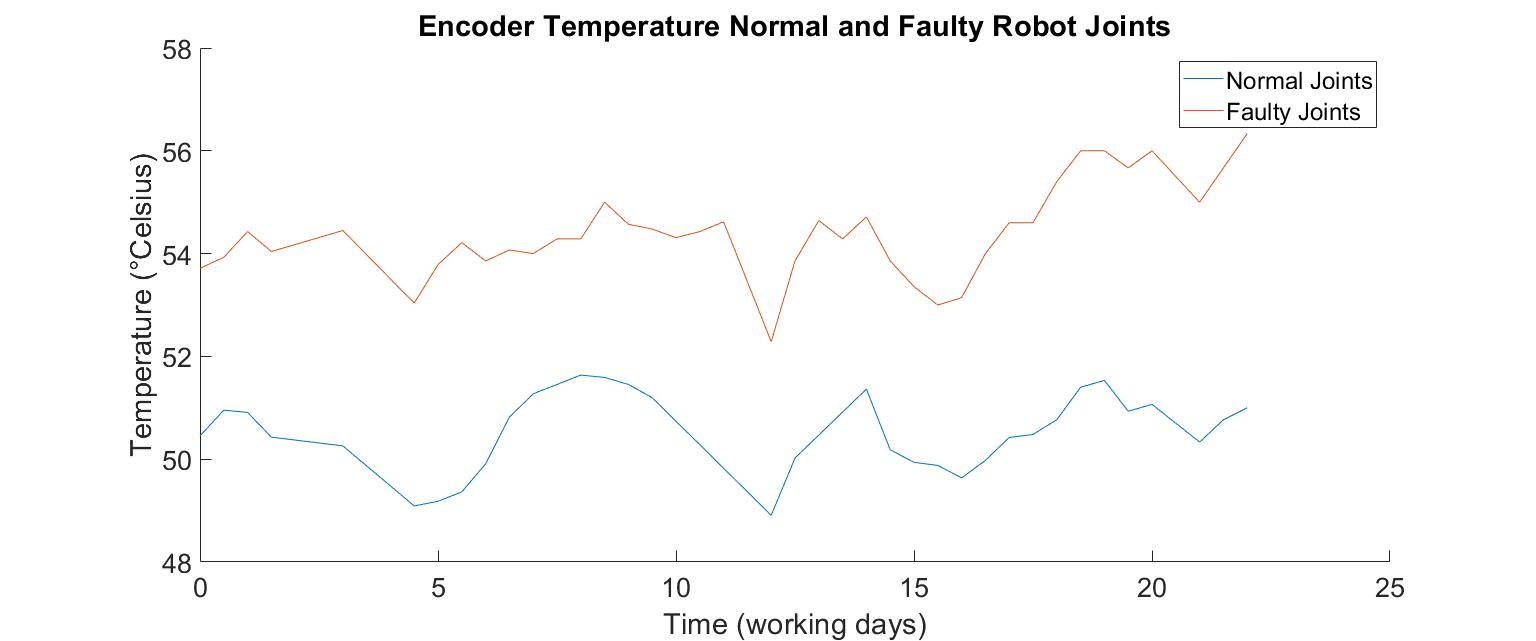
\includegraphics[width=\textwidth]{Figures/EncTemperatures}
\caption[Average encoder temperatures of normal and faulty robot arms]{Average encoder temperatures of normal and faulty robot arms} \label{fig:AvgEncTemp}
\end{figure}

According to the statements above, it is not yet conclusive that encoder temperature can indicate robot joint failure. Therefore, monitoring the temperature values will be continued daily. Afterwards, when it can be proven that encoder temperature, and perhaps more variables, can indicate robot joint failure, the model can be adjusted with implementing those variables. A Principal Component Analysis (PCA) can be useful to reduce the number of variables that are related to each other in the obtained data. It is a powerful tool for reducing the number of variables that can account for most of the variance in the data set \parencite{Virk2012}.

\subsubsection{Position Error} \label{Position Error}
As mentioned before, the position error of a robot arm joint is the difference between the commanded position and the actual position of that specific joint, also called robot joint accuracy. Once the controller receives a new input task, it have to send a commanded position to the corresponding amplifier which it then tries to reach. The height of the position error is related to the speed of the joint and the load applied to that joint. A higher speed and/or a heavier load will increase the position error \parencite{Qian1996}. According to \citet{Qiao2017} The consideration of robot joint accuracy is one of the key elements when assessing the health state of an industrial robot.

To investigate if the position error can indicate robot arm abnormality, the position errors of a proper working and a faulty robot arm are collected. The position error from the two Cobra s600's are depicted in Figure \ref{fig:HighFreqPosError}, where RA41 is the proper and RB72 is the faulty robot arm. The position errors are obtained at 1000 kHz by using the ACE software as explained in Section \ref{Software}. It can be seen that the position error peaks from RB72 are much higher than the peaks regarding RA41. The peak position error data is the highest position error that occurred since the controller is switched on. Therefore, it can occur that a peak position error has the same value as at the previous inspection.

As mentioned before, a robot arm with a higher operating speed will have higher position error peaks. It can occur that a faulty robot arm has lower position error peaks than a proper working robot arm. In other words, every robot arm has a different failure level. This failure level should therefore be threated as a variable within the intended model.
\begin{figure}[ht]
\centering
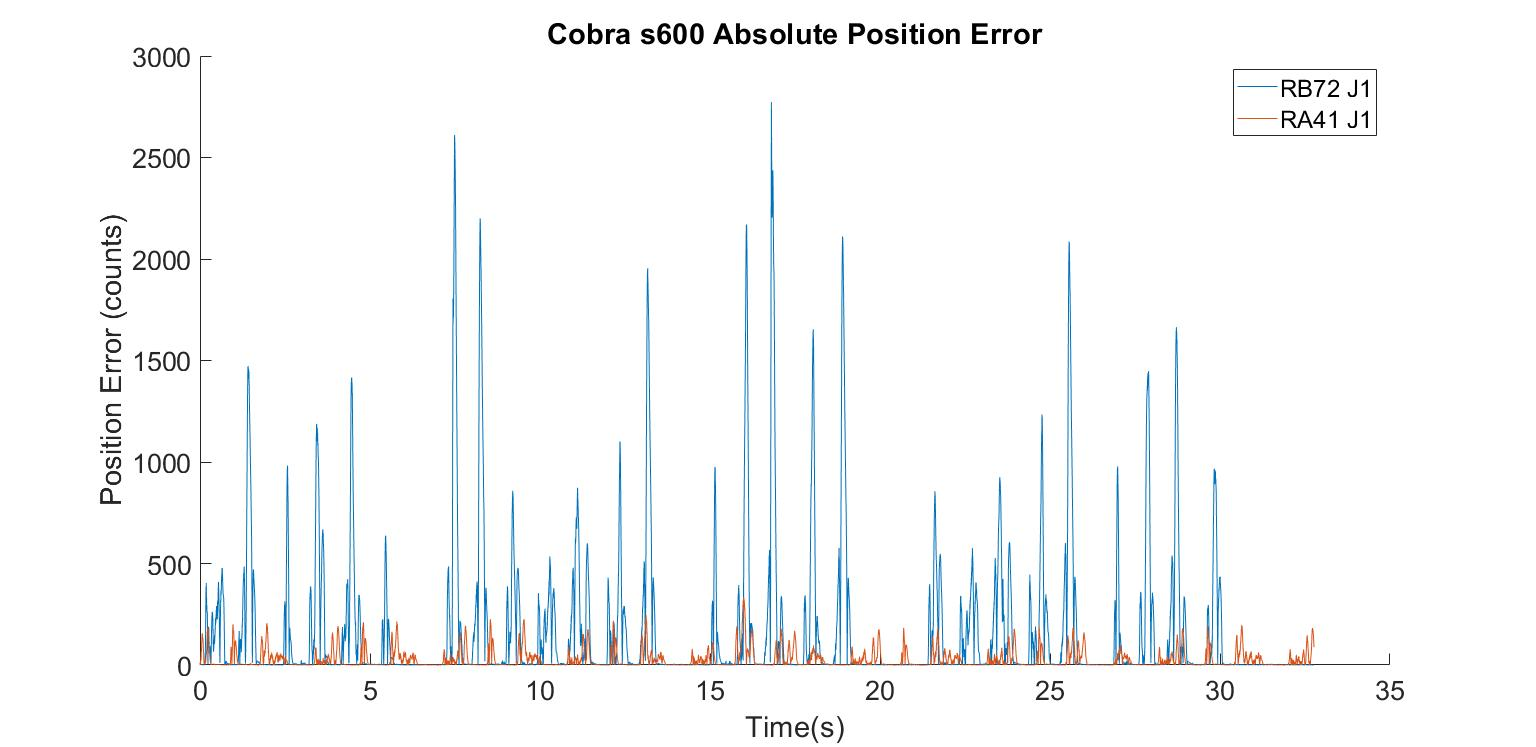
\includegraphics[width=\textwidth]{Figures/HighFreqError20}
\caption[Absolute position error for Cobra s600]{Absolute position error for Cobra s600} \label{fig:HighFreqPosError}
\end{figure}

In Figure \ref{fig:AllPosErrors}, the peak position error from several Cobra s600 robot arms are depicted. Since, the robot arms are only operating from Monday to Friday, the weekends are left out. The total time of the figure is from March 1 to March 30, or 21 working days. The red crosses indicate when a robot arm failed and was replaced by a new or revised one. As can be seen in the figure, failure at RB34 R2 J1 occurred at a lower peak position error than the failure at RB72 R1 J1. This indicates that the critical failure level differs per robot arm and a variable failure threshold should be considered. 
\begin{figure}[ht]
\centering
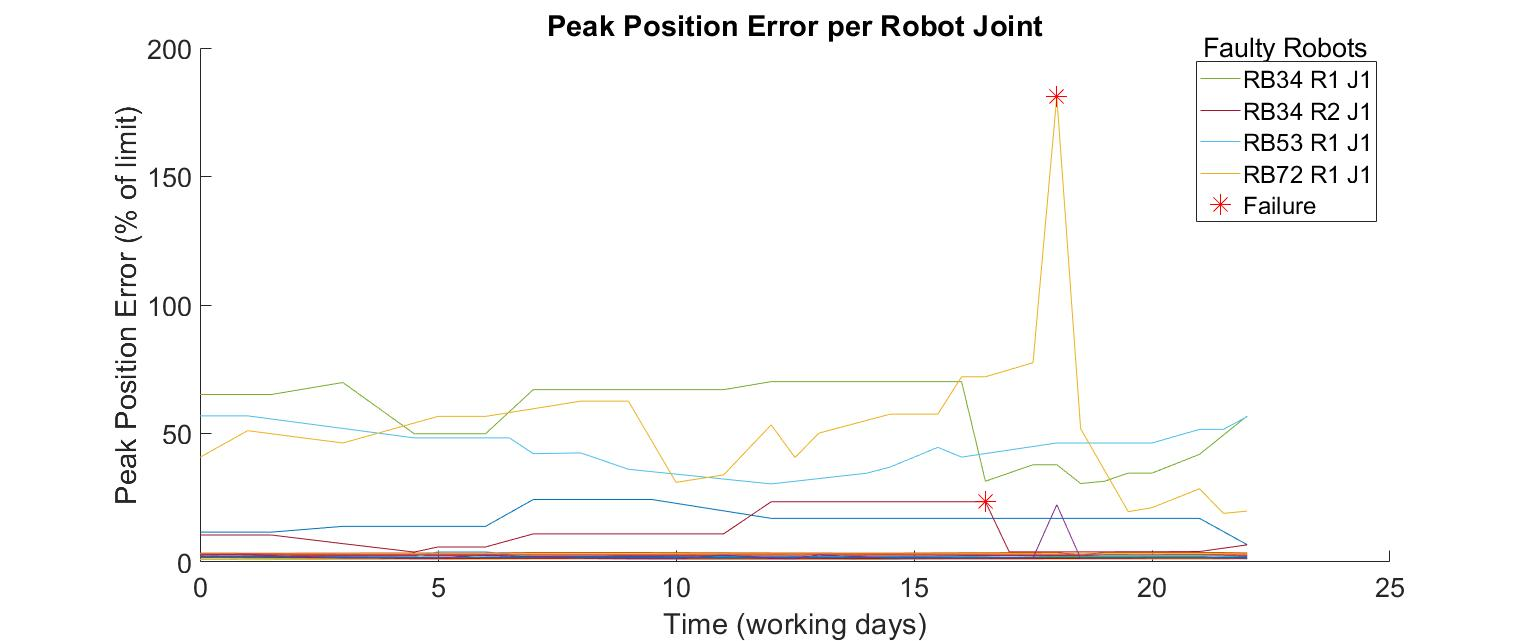
\includegraphics[width=\textwidth]{Figures/AllPeakPositionErrors20}
\caption[Peak position errors for several Cobra s600 robot arms]{Peak position errors for several Cobra s600 robot arms} \label{fig:AllPosErrors}
\end{figure}

\section{SQ2: How can the output data be interpret in order to predict maintenance?} \label{SQ2}
In the previous subsection, it was found that position error data is able to predict upcoming maintenance. Therefore, actual position error data is used to determine the path of degradation per robot arm joint. Based on this degradation path it can be predicted when the degradation has reached a critical failure level. In Figure \ref{fig:DegradationDistribution} it can be seen how the failure time should be estimated. From the known degradation path, the path left of $t$, a prediction can be achieved to determine how the degradation will evolve. The evolution of the degradation path is estimated and therefore the time to failure is also an estimate. Since that the position error data includes negative values a normal distribution for the time to failure estimation is considered. The distribution parameters, mean ($\mu$) and standard deviation ($\sigma$), are obtained for every robot arm joint separately. As concluded from the previous section, the critical failure level is different per robot arm joint and should therefore also follow a Probability Density Function (PDF).

In this subsection, it is determined how the degradation path estimation of a robot arm joint can be obtained and how the failure threshold distribution can be applied.

\begin{figure}[ht]
\centering
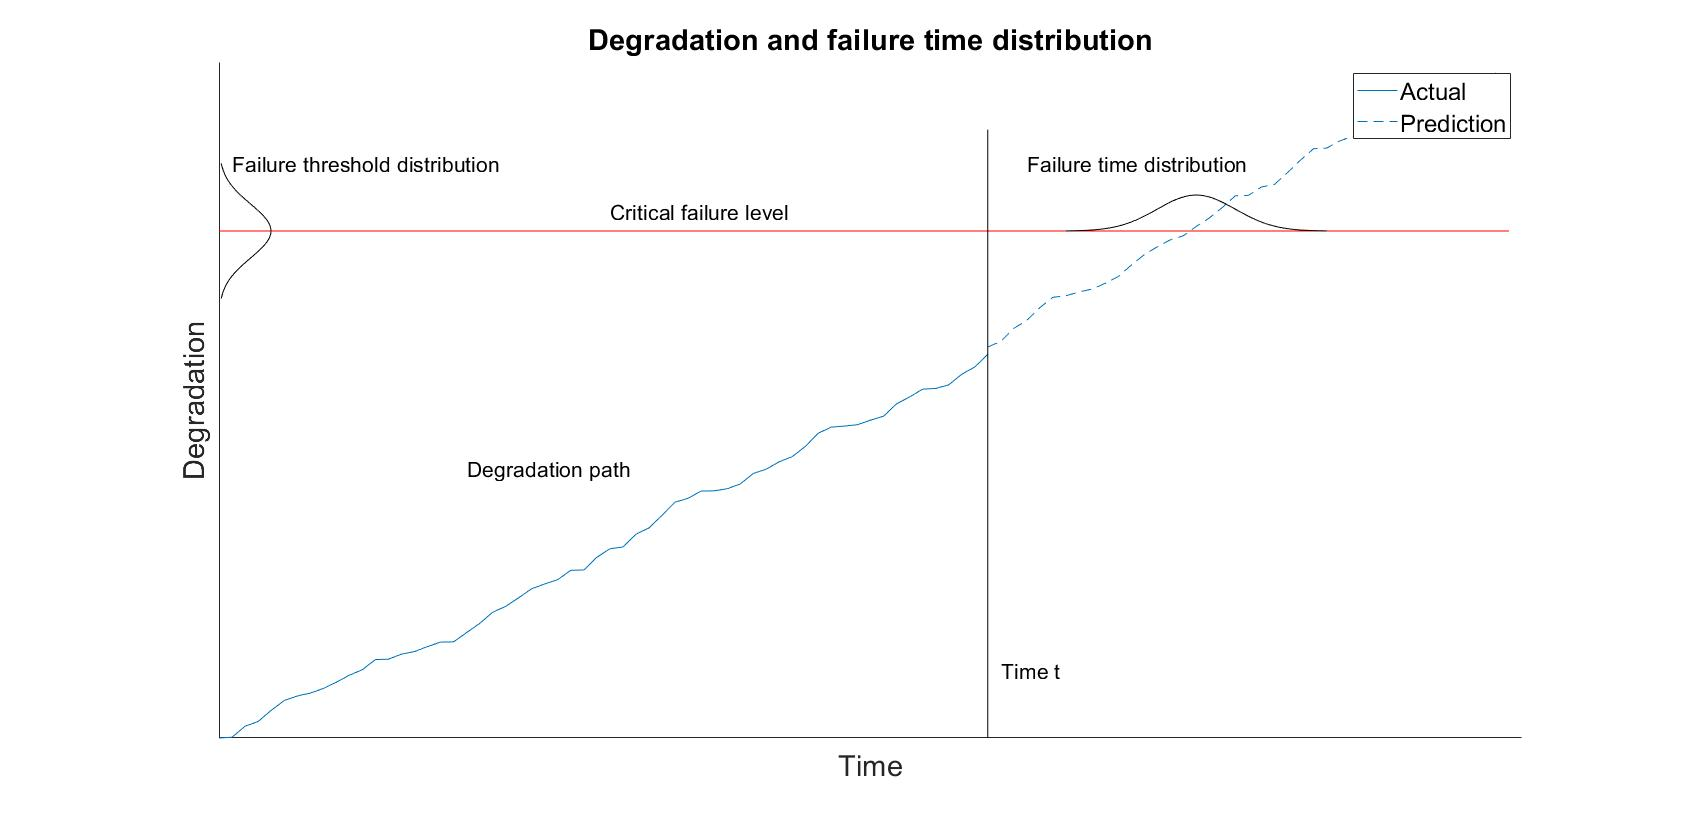
\includegraphics[width=\textwidth]{Figures/DegradationDistribution}
\caption[Degradation path and failure time distribution]{Degradation path and failure time distribution} \label{fig:DegradationDistribution}
\end{figure}

\subsection{Degradation path} \label{Degradation path}
As concluded from Section \ref{Position Error}, degradation of a robot arm joint is indicated by the position error and therefore the position error is called degradation indicator (DI). The following definitions and notations are based on the ones used by \citet{Lu1993}. The DI evolves toward the critical degradation level, or failure threshold, corresponding to the moment when the robot arm joint is no longer able to perform its designated functions. For any time, reliability of the robot arm joint can be evaluated as the probability of the DI not overshooting the failure threshold. The DI path can be described by $y_i$ over time $t$, where $y_i$ is the $i$th joint's actual DI path $\eta_i$, a function of time, plus measurement error $\varepsilon_i$. In this case the DI path is related to the peak position error as described before. When more variables to describe degradation become available, for example temperature measurements, the DI path function can be adjusted by this future variables. For this research, the peak position error is the only parameter that is used to describe the DI. Time $t$ is the number of working days (all days minus weekends and vacations). $M$ is used to denote the failure threshold. The failure time $T$ is defined as the time when the actual path $\eta$ crosses failure threshold $M$. The DI path of the $i$th robot arm joint at time $t_j$ is given by 
\begin{equation} \label{eq:degradation path}
\begin{aligned} 
	y_{ij} & = \eta_{ij} + \varepsilon_{ij} = \eta(t_j) + \varepsilon_{ij},& i & =1,2,\ldots,n, \\    
    \varepsilon_{ij} & \sim N(0,\sigma^{2}_{\varepsilon}),& j & =1,2,\ldots,m_i,
\end{aligned}
\end{equation}
where $t_j =$ time of the $j$th measurement; $\varepsilon_{ij}=$ measurement error with  standard deviation $\sigma_{\varepsilon}$; $\eta_{ij}=$ actual DI path of the $i$th joint at time $t_j$; $m_i=$ total number of inspections of the $i$th joint. \citet{Lu1993} describe that $\eta_{ij}$ has fixed and random-effect parameters denoted by $\Phi$ and $\Theta_{i}$. However, for this project it is assumed that the peak position error can indicate robot failure only and therefore $\eta_{ij}$ only consist of one parameter; peak position errors.

To give an idea how the DI path evolves in time, an example is provided in Figure \ref{fig:RB72R1J1Degradation}. It can be seen that the DI, or peak position error, increases slowly over time, on average. After the high peak around the $18$th monitored working day, it was replaced by a revised one. From here it can be seen that the DI for the revised robot arm, that execute the same task as the old one, is lower. The replaced robot arm was in operation for more than 3 years, or approximately 780 working days. The monitoring time, 25 working days, is too small to conclude anything about the actual DI path the arm underwent and assumptions have to be made. It is therefore assumed that robot arm joints degrade linearly.
\begin{figure}[ht]
\centering
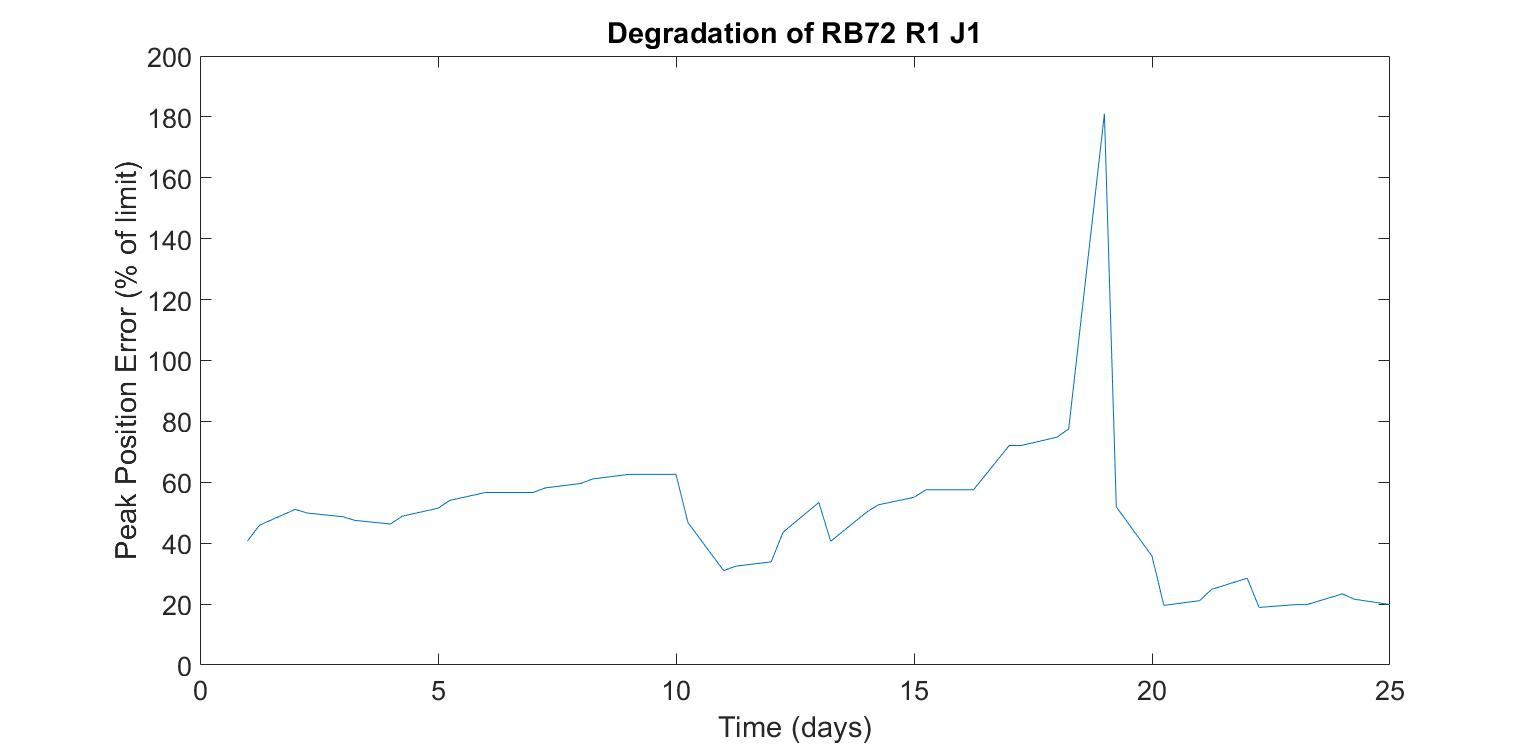
\includegraphics[width=\textwidth]{Figures/RB72R1J1Degradation}
\caption[Degradation path of RB72 Robot1 Joint 1]{Degradation path of RB72 Robot1 Joint 1} \label{fig:RB72R1J1Degradation}
\end{figure}

\subsection{Time to failure estimation} \label{TTF}
In this research the time to failure (TTF) is defined as the time between the last observation and the failure time T with respect to the degradation path. The TTF can be considered as a random variable with a probability distribution. A robot arm joint is considered to be failed when the DI cross a failure threshold, specified in the next section \ref{Random threshold}. The probability distribution function of TTF is denoted by $F_{TTF}$ is defined as follows:
\begin{equation} \label{eq:TTFeq:TTF}
F_{TTF}(t_j)=Pr[TTF \leq t_j] = \frac{1}{\sqrt[]{2\pi\sigma^2}} \int\limits_{-\infty}^{t_j} \mathrm{e}^{\frac{-(t_j-\mu)^2}{2\sigma^2}}
\end{equation}
In other words, $F_{TTF}(t_j)$ is the probability that a failure occurs in the interval $(-\infty,t_j]$ with normal distribution parameters $\mu$ and $\sigma$. This PDF is used to provide a relative likelihood that the value of the DI path will cross the threshold. 

Increments are defined as the discretized increase or decrease of the DI during a day. Since that the increments can be either positive or negative, a normal distribution is considered depicted in Figure \ref{fig:RB72R1J1PDF} for RB72 Robot1 Joint1 with $\mu=0.098292$ and $\sigma=6.4403$. Data that is used to obtain those values can be found in Appendix REF. Here, $\chi$ is the positive or negative increment size over which the peak position error can evolve per day. The obtained PDF will be different for every robot arm, since the size and frequency of increasing and decreasing position error increments will differ per arm. For this project, a fixed number of inspections is used to build the PDF and estimate a DI path prediction. However, updating the PDF is necessary to make the model more dynamic and adaptive to new input data. How this is intended will be described in Chapter \ref{Chapter6}.

\begin{figure}[ht]
\centering
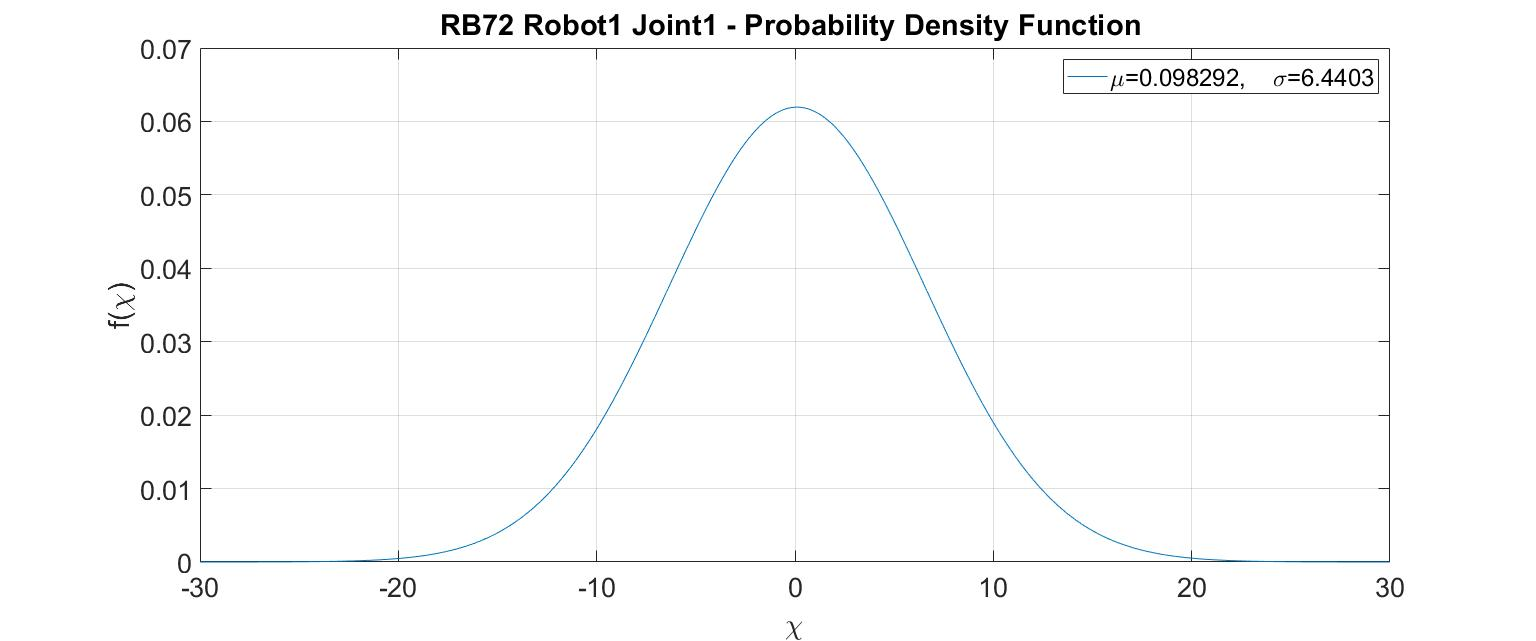
\includegraphics[width=\textwidth]{Figures/RB72R1J1PDF}
\caption[Probability density function of RB72 Robot1 Joint 1 degradation]{Probability density function of RB72 Robot1 Joint 1 degradation} \label{fig:RB72R1J1PDF}
\end{figure}

\subsection{Random deviations in failure threshold} \label{Random threshold}
\citet{Usynin2008} describe that most models used in degradation data analysis make use of the notion of a fixed critical failure threshold, in this case denoted as $M$. Since, joint failures occur at different DI values (position errors), see Section \ref{Position Error}, a probabilistic description is likely to be more appropriate. The failure threshold differs per robot and therefore a PDF that reflects the relatively vague knowledge about possible failure thresholds is used. In this case, failure threshold $M$ is defined as a range of critical values having certain probabilities. 

The following definitions and notations are based on \citet{Usynin2008}. Let $F_{M}(y)$ be the cumulative distribution function of the random critical failure threshold.
\begin{equation} \label{eq:CDF}
F_{M^*}(y)=Pr[M^*< y]
\end{equation}
where $M^*$ is the random failure threshold for degradation $y$.
\begin{equation}
f_{M^*}(y) = \frac{dF(y)}{dy}
\end{equation}
is the probability density function of the random failure threshold $M^*$. 

Only from RB72 Robot1 Joint1 and RB34 Robot2 Joint1 it is known what their failure threshold is, 70 and 25 respectively. Therefore, this PDF is constructed based on the researchers intuition and knowledge about failure levels. TBD

%Robot arms exhibit very complex dynamic behavior, and different defects can affect this behavior. Also, their motion is completely different from that of rotating machines (or other continuously moving machines), for which the majority of present condition monitoring systems have been designed. \citet{Jaber2017} describes that data subtracted from a robot arm are transitory and last for a very short time. This is in contradiction with the rotating machines discussed widely in literature that emit continuous signals during their operation. The challenge here is how to design a reliable and intelligent condition monitoring system to be able to deal with the transitory and non-transitory signals for accurate diagnosis and prognosis.Therefore, the signals captured and features extracted have to be analyzed and classified in an appropriate way to provide an unambiguous identification of a faulty robot part before a catastrophic failure occurs.

%Currently, the OTD of Philips uses direct inspection to measure the condition of robot arms and to find defective faults. By applying CBM, these direct inspections should be replaced by condition monitoring using sensors within the robot arm. In Section \ref{SQ1}, it is determined what data types should be analyzed to achieve a reliable maintenance prediction. 

\section{SQ3: On what performance indicators should the artifact be evaluated?} \label{SQ3}
The DI path $y$ \ref{eq:degradation path} and probability density functions $f_{M^*}$ \ref{eq:CDF} and $F_{T}$ REF should be checked on their correctness. Since the monitoring time of the robot arms is relatively small, as discussed in the previous section, a simulation is performed besides an experiment to check the appropriateness of the PDF based model. 

\subsection{Experiment} \label{Experiment}
In this section, the model is tested on new real experiment data available from robot arms to check whether the model is able to determine when it will cross the failure threshold. Data available 

\subsection{Simulation} \label{Simulation}
By performing simulations, the model can be tested how it will contribute to the maintenance schedule at Philips. 

\subsection{Comparison of experiment and simulation} \label{ExpvsSim}
The results of the experiment and the simulation will be discussed and compared.

\section{SQ4: What are requirements for software engineers to integrate the artifact in the control system?} \label{SQ4}
The validated model should be implemented into the RB34 and later in other RACs and therefore software requirements should be determined. Maybe a conversation with Frank Velthuis, a software engineer from Beenen, will bring some new insights forward. TBD

\chapter{Evaluation} \label{Chapter6}

%----------------------------------------------------------------------------------------
%	THESIS CONTENT - APPENDICES
%----------------------------------------------------------------------------------------
\appendix % Cue to tell LaTeX that the following "chapters" are Appendices
% Appendix A

\chapter{Frequently Asked Questions} % Main appendix title

\label{AppendixA} % For referencing this appendix elsewhere, use \ref{AppendixA}

\section{How do I change the colors of links?}

The color of links can be changed to your liking using:

{\small\verb!\hypersetup{urlcolor=red}!}, or

{\small\verb!\hypersetup{citecolor=green}!}, or

{\small\verb!\hypersetup{allcolor=blue}!}.

\noindent If you want to completely hide the links, you can use:

{\small\verb!\hypersetup{allcolors=.}!}, or even better: 

{\small\verb!\hypersetup{hidelinks}!}.

\noindent If you want to have obvious links in the PDF but not the printed text, use:

{\small\verb!\hypersetup{colorlinks=false}!}.

\chapter{Data Collection Parameters} \label{AppendixB}
\begin{table}[ht]
\begin{center}
\caption[Parameter types available from the SmartController regarding the robot]{Parameter types available from the SmartController regarding the robot} \vspace{0.3cm}
\label{tab:Robot Data Types}
\begin{tabular}[width=\textwidth]{ p{0.33\textwidth} | p{0.62\textwidth}}
Parameter & Description \\ [1ex]
\hline \\
\parbox[t]{0.3\textwidth}{Bus Voltage} & The current amplifier bus voltage for the robot. \\ [2ex]
\parbox[t]{0.3\textwidth}{AC Input} & The current AC input voltage (220 VAC) for the robot. \\ [2ex]
\parbox[t]{0.3\textwidth}{DC Input} & The current DC input voltage (24 VDC) for the robot.\\ [2ex]
\parbox[t]{0.3\textwidth}{Base Board Temperature} &  The current temperature (in $^\circ$C) for the amp-in-base processor board. \\
\end{tabular}
\end{center}
\end{table}

\begin{longtable}[width=\textwidth]{ p{0.33\textwidth} | p{0.62\textwidth}}
\caption[Parameter types available from the SmartController regarding the motors]{Parameter types available from the SmartController regarding the motors} \vspace{0.3cm}
\label{tab:Motor Data Types} \\
Parameter & Description \\ [1ex]
\hline \\
\parbox[t]{0.33\textwidth}{Amp AC Input} & Monitors the RMS input voltage to amplifier (in volts) for the selected motor.\\ [2ex]
\parbox[t]{0.33\textwidth}{Amp Bus} & Monitors the high-voltage DC bus (in volts) for the selected motor.\\ [2ex]
\parbox[t]{0.33\textwidth}{Amp Temperature} & Monitors the amplifier temperature (in $^\circ$C) for the selected motor.\\ [2ex]
\parbox[t]{0.33\textwidth}{Amplifier Temperature} & The current temperature (in $^\circ$C) for the motor amplifier. This should not exceed the specified limits. \\ [2ex]
\parbox[t]{0.33\textwidth}{Base Board Temperature} & Monitors the amplifier base-board temperature (in $^\circ$C), per-amp not per motor, for the selected motor.\\ [2ex]
\parbox[t]{0.33\textwidth}{Bus Energy Filter} & Monitors the Bus Energy Filter for the selected motor.\\ [2ex]
\parbox[t]{0.33\textwidth}{Commanded Acceleration} & Monitors the commanded acceleration (in counts/ms$^2$) for the selected motor.\\ [2ex]
\parbox[t]{0.33\textwidth}{Commanded Position} & Monitors the commanded position (in counts) for the selected motor. \\ [2ex]
\parbox[t]{0.33\textwidth}{Commanded Velocity} & Monitors the commanded velocity (in counts/ms) for the selected motor.\\ [2ex]
\parbox[t]{0.33\textwidth}{Current Loop Output} & Monitors the output of the 'PI' current loop for the selected motor.\\ [2ex]
\parbox[t]{0.33\textwidth}{Current Peak-to-Peak Output} & Monitors the peak output of the 'PI' current loop for the selected motor.\\ [2ex]
\parbox[t]{0.33\textwidth}{DC Input Voltage} & Monitors the DC control voltage (in volts) for the selected motor\\ [2ex]
\parbox[t]{0.33\textwidth}{Duty Cycle} & The current duty cycle value, as a percentage, for the selected motor. \\ [2ex]
\parbox[t]{0.33\textwidth}{Duty Cycle Limit} & Specifies the maximum allowable value for the Duty Cycle. When Duty Cycle Level = Duty Cycle Limit, the robot is stopped to protect the motor. See Duty Cycle Level and Peak Duty Cycle. \\ [2ex]
\parbox[t]{0.33\textwidth}{Encoder Position} & Monitors the actual position (in counts) for the selected motor.\\ [2ex]
\parbox[t]{0.33\textwidth}{Encoder Temperature} & Monitors the encoder temperature (in $^\circ$C) for the selected motor.\\ [2ex]
\parbox[t]{0.33\textwidth}{Encoder Velocity} & Monitors the actual velocity, in counts/ms, for the selected motor.\\ [2ex]
\parbox[t]{0.33\textwidth}{E-Stop Status} & Monitors the E-stop status register for the selected motor.\\ [2ex]
\parbox[t]{0.33\textwidth}{Index Delta} & Monitors the index delta (last index position minus previous index position), in counts, for the selected motor. \\ [2ex]
\parbox[t]{0.33\textwidth}{Last Motion Settling Time} & Monitors the motor settling time (in milliseconds) of the last motion completed for the selected motor.\\ [2ex]
\parbox[t]{0.33\textwidth}{Latched Errors} & Monitors the latched error bit mask for the selected motor. For possible values and their descriptions, see the topic MotorLatchedErrorBits Enumeration in the ACE API Documentation Help file. You can access this file by selecting Help > ACE API Reference from the ACE software menu. \\ [2ex]
\parbox[t]{0.33\textwidth}{Output Level} & Monitors the output level, typically a torque command between -32768 and 32767, for the selected motor.\\ [2ex]
\parbox[t]{0.33\textwidth}{Peak Duty Cycle} & Monitors the largest Duty Cycle value that has been reached since the last controller boot. This allows you to see if the robot is approaching the Duty Cycle Limit. See Duty Cycle Level and Duty Cycle Limit.\\ [2ex]
\parbox[t]{0.33\textwidth}{Peak Position Error} & The peak position error, as a percentage of soft envelope error, for the selected motor.\\ [2ex]
\parbox[t]{0.33\textwidth}{Peak Torque} & The peak torque, as a percentage based on maximum torque, for the selected motor.\\ [2ex]
\parbox[t]{0.33\textwidth}{Position Error} & Monitors the position error (commanded position minus actual encoder position), in counts, for the selected motor. \\ [2ex]
\parbox[t]{0.33\textwidth}{Servo Status} & Monitors the servo status bit mask for the selected motor. For possible values and their descriptions, see the topic MotorStatusBits Enumeration in the ACE API Documentation Help file. You can access this file by selecting Help > API Reference from the ACE software menu.\\ [2ex]
\parbox[t]{0.33\textwidth}{Unlatched Errors} & Monitors the unlatched error bit mask for the selected motor. For possible values and their descriptions, see the topic MotorUnlatchedErrorBits Enumeration in the ACE API Documentation Help file. You can access this file by selecting Help > API Reference from the ACE software menu. \\ [2ex]
\parbox[t]{0.33\textwidth}{Velocity Error} & Monitors the velocity error (commanded velocity minus encoder velocity), in counts/ms, for the selected motor. \\ [2ex]
\end{longtable}
% Appendix Template

\chapter{Design Project Planning} \label{AppendixC}
The execution of the research is planned to last 18 working weeks, November 24th - April 27th including 2 weeks vacations and 1 week of studying for a course. This time will be divided in three parts: Firstly the Problem Analysis, Literature study and Research Design will be performed. Secondly, the research execution is performed and a artifact will be designed. Lastly, the report will be finalized and a presentation is given about the project. The planning is shown in a Gantt Chart, depicted in Figure \ref{fig:Planning}, where the performed steps are deleted. During the execution of the project, adjustments can be made regarding the planning. Therefore, the planning will be updated for every hand-in moment and will be excluded in the final version.
\begin{figure}[ht]
\centering
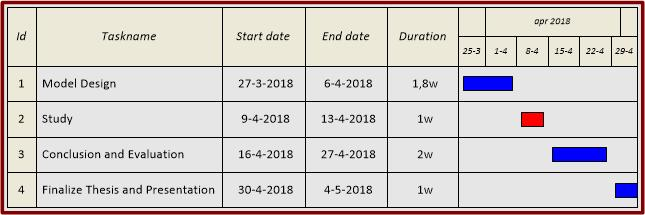
\includegraphics[width=\textwidth]{Figures/Research_Planning2}
\caption{Design Project Planning}
\label{fig:Planning}
\end{figure}
%----------------------------------------------------------------------------------------

%	BIBLIOGRAPHY
\printbibliography[heading=bibintoc]

\end{document}  
